\documentclass{thesis/PatternRecognition}
\usepackage{thesis/scnu}
\usepackage{thesis/mynewcommand}
\usepackage{listings}
\usepackage{xcolor}
\usepackage{color}
\usepackage{multirow}
\usepackage{booktabs}
\usepackage{enumerate}
\usepackage{amsmath}

\graphicspath {{figures/}}%The folder containing pictures
\captionsetup{font={footnotesize}}
\definecolor{darkgreen}{rgb}{0,0.6,0}
\definecolor{underground}{rgb}{0.949,0.949,0.949}
\definecolor{strcolor}{rgb}{0.8,0,0.8}
\colorlet{stringcolour}{red!60!black}
\colorlet{keywordcolour}{magenta!90!black}
\colorlet{exceptioncolour}{yellow}
\colorlet{commandcolour}{blue!60!black}
\colorlet{numpycolour}{blue!60!green}
\colorlet{literatecolour}{magenta!90!black}
\colorlet{promptcolour}{green!50!black}
\colorlet{specmethodcolour}{violet}
\colorlet{commentcolour}{green!50!black}

\numberwithin{eqnarray}{section}


\begin{document}

\lstset
{
language=python,
numbers=left,
numberstyle=\color{blue}, 						%代码编号
%stepnumber=0,									%代码编号步长
keywordstyle=\color{keywordcolour}\bfseries,			%关键字颜色
commentstyle=\color{commentcolour},					%注释颜色
%frame=shadowbox,								%边框
breaklines=true, 								%自动折行
stringstyle=\color{stringcolour},				%字符串颜色
backgroundcolor=\color{underground},			%背景色
xleftmargin=0cm,xrightmargin=0cm, aboveskip=1cm, %设置边距
basicstyle=\small,								%基本字体字号  
rulesepcolor=\color{red!20!green!20!blue!20},
flexiblecolumns=true, 
breakautoindent=true,
%python特有关键字
emph={and,break,class,continue,def,yield,del,elif ,else,%
except,exec,finally,for,from,global,if,import,in,%
lambda,not,or,pass,print,raise,return,try,while,assert,with},
emphstyle=\color{blue}\bfseries,
emph={[2]True, False, None},
emphstyle=[2]\color{keywordcolour},
emph={[3]object,type,isinstance,copy,deepcopy,zip,enumerate,reversed,list,len,dict,tuple,xrange,append,execfile,real,imag,reduce,str,repr},
emphstyle=[3]\color{commandcolour},
emph={Exception,NameError,IndexError,SyntaxError,TypeError,FileNotFoundError,ValueError,OverflowError,ZeroDivisionError},
emphstyle=\color{exceptioncolour}\bfseries ,
emph={[4]ode, fsolve, sqrt, exp, sin, cos,arctan, arctan2, arccos, pi,  array, norm, solve, dot, arange, , isscalar, max, sum, flatten, shape, reshape, find, any, all, abs, plot, linspace, legend, quad, polyval,polyfit, hstack, concatenate,vstack,column_stack,empty,zeros,ones,rand,vander,grid,pcolor,eig,eigs,eigvals,svd,qr,tan,det,logspace,roll,min,mean,cumsum,cumprod,diff,vectorize,lstsq,cla,eye,xlabel,ylabel,squeeze},
emphstyle=[4]\color{numpycolour},
emph={[7]range},
emphstyle={[7]\color{keywordcolour}\bfseries},
emph={[8]1, 2, 3, 4, 5, 6, 7, 8, 9, 0},
emphstyle={[8]\color{keywordcolour}\bfseries},
}



		\ctitle{机器学习笔记}
		\begin{center}
		张泓铨\ 华南师范大学\\
		龙阳扬\ 华南师范大学
		\end{center}


\pagestyle{fancy}
\rhead{}
\chead{CS229笔记}
\lhead{}
\cfoot{}
\rfoot{\thepage}



\tableofcontents       %输出目录
\newpage
\section{线性回归与梯度下降}
\subsection{符号说明}
\begin{center}
\begin{tabular}{cc}
\toprule[2pt]
变量 & 含义 \\ 
\midrule[1pt]
$x^{(i)}$ & 第$i$个特征输入(features) \\ 
$y^{(i)}$ & 第$i$个目标输出(target) \\ 
$(x^{(i)},y^{(i)})$ & 第$i$个训练样本 \\ 
$\mathbf{X}$ & 输入向量空间,为列向量 \\ 
$\mathbf{y}$ & 输出变量 \\ 
$m$ & 数据样本个数 \\
$n$ & 输入变量的特征个数\\
$\theta$ & 参数向量,为列向量\\
\bottomrule[2pt]
\end{tabular}
\end{center}


\subsection{线性回归}
考虑线性函数
\begin{eqnarray}
h_\theta(x)=\theta_0+\theta_1x_1+\theta_2x_2+\cdots+\theta_nx_n
\end{eqnarray}
为了简化$h_\theta(x)$,将$x_0=1$引入,令$\mathbf{\theta(x)}=(\theta_0,\theta_1,\cdots,\theta_n)^T$,则有
\begin{eqnarray}
h_\theta(x)
&=&\sum_{i=0}^n\theta_ix_i\\
&=&
\begin{pmatrix}
\theta_0&\theta_1&\cdots & \theta_n
\end{pmatrix}
\begin{pmatrix}
1\\
x_1\\
\vdots\\
x_n
\end{pmatrix}\\
&=&\mathbf{\theta}^Tx
\end{eqnarray}
定义损失函数
\begin{eqnarray}
J(\theta)=\frac{1}{2}\sum_{i=1}^m(h_\theta(x^{(i)})-y^{(i)})^2
\end{eqnarray}
该方法被称为普通最小二乘方法(ordinary least squares)。其中,增加系数$\frac{1}{2}$是为了求导方便,而不影响其方向。
\subsection{LMS与梯度下降法}
为了通过最小化误差函数$J(\theta)$来求解最优的$\theta$。其中一个方法是采用梯度下降法。梯度下降法采用迭代$\theta$来使得$J(\theta)$变小,直到达到一定的值之后停止迭代。该算法任意初始化一个$\theta$,通过如下方式更新
\begin{eqnarray}
\theta_j := \theta_j-\alpha\frac{\partial}{\partial \theta_j}J(\theta)
\end{eqnarray}
其中,$\alpha$为学习率(learning rate),决定每次迭代的调整尺度。若对单个的训练样本$(x^{(i)},y^{(i)})$,计算$J(\theta)$的偏导,有
\begin{eqnarray}
\frac{\partial}{\partial \theta_j}
&=&\frac{\partial}{\partial \theta_j}\frac{1}{2}(h_\theta(x^{(i)})-y^{(i)})^2\\
&=&(h_\theta(x^{(i)})-y^{(i)})\frac{\partial}{\partial\theta_j}(h_\theta(x^{(i)})-y^{(i)})\\
&=&(h_\theta(x)-y^{(i)})\frac{\partial}{\partial\theta_j}
\left(
\begin{aligned}
\sum_{i=1}^n\theta_ix^{(i)}_i-y^{(i)}
\end{aligned}
\right)\\
&=&(h_\theta(x^{(i)})-y^{(i)})x_j
\end{eqnarray}
因而,其更新规则为
\begin{eqnarray}
\theta_j:=\theta_j+\alpha(y^{(i)}-h_\theta(x^{(i)}))x^{(i)}_j
\end{eqnarray}
该规则被称为LMS(least mean squares)。在迭代过程中,通常不会选择大的学习率,因其会产生过拟合的情况,或产生在最优解附近震荡。一般情况下,对$J(\theta)$的最优值求解是二次规划问题,是有最优解的。假设$m$是数据样本个数,梯度下降法考虑遍历所有数据样本之后,在对参数$\mathbf{\theta}$进行更新,公式如下
\begin{eqnarray}
\theta_j:=\theta_j+\alpha\sum_{i=1}^m(y^{(i)}-h_\theta(x^{(i)}))x_j^{(i)}
\end{eqnarray}
由于这种更新方式需要遍历所有的数据样本,其迭代速度会比较慢,以下两种方法是对梯度下降法的改进算法。
\subsection{随机梯度下降法(incremental gradient descent)}
在样本中随机抽取一个样本,并采取式(11)调整$\theta_j$,循环直到误差值符合收敛条件。这种算法是对梯度下降法的改进,其对抽取的一个样本便进行调整,而无需式(12)进行遍历,计算速度会显著加快。但因其采用片面的数据作调整,其调整的梯度有可能并非是最优方向,因而其有可能会陷入局部最优解,且需要更多次迭代来达到收敛条件。
\subsection{批量梯度下降法(batch gradient descnet)}
这是一种对于梯度下降法和随机梯度下降法的这种方法。假设采集批量为$p$,则在数据集中做$p$次采样,拓展成一个有$p$个样本的数据集,通过式(12)来更新$\theta$。此方法常会取得好的效果。
\subsection{线性回归的显式求解}
设矩阵$A=
\begin{pmatrix}
a_{11} & \cdots & a_{1n}\\
\vdots & \ddots & \vdots\\
a_{m1} & \cdots & a_{mn}
\end{pmatrix}
$
,
$B=
\begin{pmatrix}
b_{11} & \cdots & b_{1n}\\
\vdots & \ddots & \vdots\\
b_{m1} & \cdots & b_{mn}
\end{pmatrix}
$
,$\textbf{tr}(A)$为矩阵$A$的迹,即对角线上元素之和,$a\in \mathbb{R}$,函数$f$定义为$f(A)=AB$,
则有如下结论
\begin{eqnarray}
\textbf{tr}AB&=&\textbf{tr}BA\\
\textbf{tr}ABC&=&\textbf{tr}CAB = \textbf{tr}BCA\\
\textbf{tr}A&=&\textbf{tr}A^T\\
\textbf{tr}(A+B)&=&\textbf{tr}A+\textbf{tr}B\\
\textbf{tr}aA&=&a\textbf{tr}A\\
\nabla_{A}\textbf{tr}AB &=& B^T\\
\nabla_A \textbf{tr}(ABA^TC) &=& CAB+C^TAB^T\\
\nabla_{A^T}f(A)&=&(\nabla_Af(A))^T\\
\nabla_A|A|&=&|A|(A^{-1})
\end{eqnarray}
我们将第$i$个样本的输入记为$x^{(i)}$,其为列向量:
\begin{eqnarray}
x^{(i)}=(x^{(i)}_1,x^{(i)}_2,\cdots,x^{(i)}_n)^T
\end{eqnarray}
则样本输入可表示为
\begin{eqnarray}
X=
\begin{pmatrix}
(x^{(1)})^T\\
(x^{(2)})^T\\
\vdots\\
(x^{(n)})^T
\end{pmatrix}
\end{eqnarray}
将样本输出记为
\begin{eqnarray}
Y=
\begin{pmatrix}
y^{(1)}\\
y^{(2)}\\
\vdots\\
y^{(n)}
\end{pmatrix}
\end{eqnarray}

由于$\theta$为列向量,因而有
\begin{eqnarray}
\begin{aligned}
X\theta-Y
&=
\begin{pmatrix}
(x^{(1)})^T\theta\\
(x^{(2)})^T\theta\\
\vdots\\
(x^{(m)})^T\theta
\end{pmatrix}
-
\begin{pmatrix}
y^{(1)}\\
y^{(2)}\\
\vdots\\
y^{(m)}
\end{pmatrix}\\
&=
\begin{pmatrix}
(x^{(1)})^T\theta-y^{(1)}\\
(x^{(2)})^T\theta-y^{(2)}\\
\vdots\\
(x^{(m)})^T\theta-y^{(m)}
\end{pmatrix}
\end{aligned}
\end{eqnarray}
由于对于列向量$z$,有$z^Tz=\sum_iz_i^2$,因而有
\begin{eqnarray}
\begin{aligned}
J(\theta)&=\frac{1}{2}\sum_{i=1}^m(h_\theta(x^{(i)})-y^{(i)})^2\\
&= \frac{1}{2}(X\theta-Y)^T(X\theta-Y)\end{aligned}
\end{eqnarray}
因而有
\begin{eqnarray}
\begin{aligned}
\nabla_\theta J(\theta)&=\nabla_\theta\frac{1}{2}\sum_{i=1}^m(h_\theta(x^{(i)})-y^{(i)})^2\\
&=\frac{1}{2}\nabla_\theta((X\theta)^T(X\theta)-(X\theta)^TY-Y^T(X\theta)-Y^TY)\\
&=\frac{1}{2}\nabla_\theta(\theta^TX^TX\theta-\theta^TX^TY-Y^TX\theta-Y^TY)\\\end{aligned}
\end{eqnarray}
由于$\theta^TX^TX\theta-\theta^TX^TY-Y^TX\theta-Y^TY$为数,即$1\times1$的矩阵,因而有
\begin{eqnarray}
\begin{aligned}
\theta^TX^TX\theta-\theta^TX^TY-Y^TX\theta-Y^TY=\textbf{tr}(\theta^TX^TX\theta-\theta^TX^TY-Y^TX\theta-Y^TY)
\end{aligned}
\end{eqnarray}
所以有
\begin{eqnarray}
\begin{aligned}
\nabla_\theta J(\theta)
 &=\frac{1}{2}\nabla_\theta(\theta^TX^TX\theta-\theta^TX^TY-Y^TX\theta-Y^TY)\\
&=\frac{1}{2}\nabla_\theta\textbf{tr}(\theta^TX^TX\theta-\theta^TX^TY-Y^TX\theta-Y^TY)\\
&=\frac{1}{2}\nabla_\theta(\textbf{tr}\theta^TX^TX\theta-\textbf{tr}\theta^TX^TY-\textbf{tr}Y^TX\theta+\textbf{tr}Y^TY)
\end{aligned}
\end{eqnarray}
由于$\textbf{tr}AB=\textbf{tr}BA$,因而有$\textbf{tr}\theta^TX^TY=\textbf{tr}Y^TX\theta$,且$\nabla_\theta\textbf{tr}Y^TY=0$,于是有
\begin{eqnarray}
\begin{aligned}
\nabla_\theta J(\theta)&=\frac{1}{2}\nabla_\theta(\textbf{tr}\theta^TX^TX\theta-2\textbf{tr}Y^TX\theta)\\
&=\frac{1}{2}(X^TX\theta+X^TX\theta-2X^TY)\\
&=X^TX\theta-X^TY
\end{aligned}
\end{eqnarray}
令$\nabla_\theta J(\theta)=X^TX\theta-X^TY=0$,则可得到
$X^TX\theta-X^TY$
一般情况下,$X^TX$为可逆矩阵,因而有
\begin{eqnarray}
\theta=(X^TX)^{-1}X^TY
\end{eqnarray}

\subsection{采取最小平方误差作为损失函数的原因}
在做回归的过程中,常采用最小平方误差作为损失函数,即
\begin{eqnarray}
J(\theta)=\frac{1}{2}\sum_{i=1}^m(h_\theta(x^{(i)})-y^{(i)})^2
\end{eqnarray}
假设第$i$个样本误差为$\epsilon^{(i)}$,$y^{(i)}$为实际值,$\hat{y}_i$为预测值,则有
\begin{eqnarray}
y^{(i)}&=&\hat{y}_i+\epsilon^{(i)}\\
&=&\theta^Tx^{(i)}+\epsilon^{(i)}
\end{eqnarray}
假设$\epsilon^{(i)}$为独立同分布,由大数定律,可将$\epsilon^{(i)}$假设为服从正态分布$\epsilon^{(i)}\sim \mathcal{N}(0,\sigma^2)$,因而有下式成立
\begin{eqnarray}
p(\epsilon^{(i)})=\frac{1}{\sqrt{2\pi}\sigma}\exp
\left(
-\frac{(\epsilon^{(i)})^2}{2\sigma^2}
\right)
\end{eqnarray}
则可以得到在给定$\theta$,$x^{(i)}$下得到$y^{(i)}$的概率,即预测准确的概率
\begin{eqnarray}
p(y^{(i)}|x^{(i)};\theta)=\frac{1}{\sqrt{2\pi}\sigma}\exp
\left(
-\frac{(y^{(i)}-\theta^Tx^{(i)})^2}{2\sigma^2}
\right)
\end{eqnarray}
定义似然函数
\begin{eqnarray}
\begin{aligned}
L(\theta)&=L(\theta;X,Y)\\
&=p(Y|X;\theta)\\
&=\prod_{i=1}^m p(y^{(i)}|x^{(i)};\theta)\\
&=\prod_{i=1}^m \frac{1}{\sqrt{2\pi}\sigma}\exp
\left(
-\frac{(\epsilon^{(i)})^2}{2\sigma^2}
\right)
\end{aligned}
\end{eqnarray}
为了使预测准确的概率尽可能高,则转化为$\theta$下的最大化似然函数。一般情况下,可将最大化似然函数问题转化为最大化对数似然函数的问题。
\begin{eqnarray}
\begin{aligned}
l(\theta) &= \log L(\theta)\\
&=\log \prod_{i=1}^m \frac{1}{\sqrt{2\pi}\sigma}\exp
\left(
-\frac{(\epsilon^{(i)})^2}{2\sigma^2}
\right)\\
&= \sum_{i=1}^m\log \frac{1}{\sqrt{2\pi}\sigma}\exp
\left(
-\frac{(\epsilon^{(i)})^2}{2\sigma^2}
\right)\\
&= m\log\frac{1}{\sqrt{2\pi}\sigma}-\frac{1}{\sigma^2}\cdot\frac{1}{2}\sum_{i=1}^m(y^{(i)}-\theta^Tx^{(i)})^2
\end{aligned}
\end{eqnarray}
由于其他量为常数,只有下式起作用
\begin{eqnarray}
\frac{1}{2}\sum_{i=1}^m(y^{(i)}-\theta^Tx^{(i)})^2
\end{eqnarray}
该形式与最小平方误差相同。

\subsection{局部加权线性回归}
局部加权回归是一种非参数方法,其可以根据样本量决定所需的参数个数,因而可以减少人为选择参数个数的工作量。局部加权线性回归的思想是对点周边的值赋予较大的权重,而对于较远的值赋较小的权重。该权重位于误差函数,即
\begin{eqnarray}
\min_\theta \sum_{i=1}^mw^{(i)}(y^{(i)}-\theta^Tx^{(i)})^2
\end{eqnarray}
为使权重符合要求,权重可以为如下形式
\begin{eqnarray}
w^{(i)}=\exp
\left(
\begin{aligned}
-\frac{(x^{(i)}-x)^2}{2\tau^2}
\end{aligned}
\right)
\end{eqnarray}



\section{logistic回归}
\subsection{梯度下降与logistic回归}
对于二分类问题,常采用logistic回归。若采用线性回归做二分类预测问题,其预测取值有可能大于1或小于0。为了解决这个问题,在$\theta^Tx$增加logistic函数变换(或称为sigmoid函数变换)
\begin{eqnarray}
h_\theta(x)=g(\theta^Tx)=\frac{1}{1+e^{-\theta^Tx}}
\end{eqnarray}
其中
\begin{eqnarray}
g(z)=\frac{1}{1+e^{-x}}
\end{eqnarray}
称为logistic函数或者sigmoid函数。其函数图像如下
\begin{center}
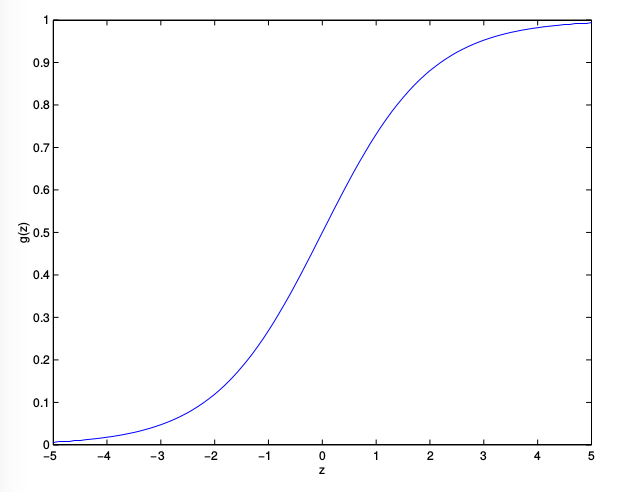
\includegraphics[scale=0.5]{../figures/cs229_2_1.png} 
\end{center}
该函数的求导结果为
\begin{eqnarray}
\begin{aligned}
g'(z) &= \frac{d}{dz}\frac{1}{1+e^{-x}}\\
&= \frac{1}{(1+e^{-z})^2}(e^{-z})\\
&= \frac{1}{1+e^{-z}}
\left(
\begin{aligned}
1-\frac{1}{(1+e^{-z})}
\end{aligned}
\right)\\
&= g(z)(1-g(z))
\end{aligned}
\end{eqnarray}
准确概率可以如下表示
\begin{eqnarray}
P(y=1|x;\theta) &=& h_\theta(x)\\
P(y=0|x;\theta) &=& 1-h_\theta(x)
\end{eqnarray}
将上式结合起来,有
\begin{eqnarray}
p(y|x;\theta)=(h_\theta(x))^y(1-h_\theta(x))^{1-y}
\end{eqnarray}
则似然函数可以表示为
\begin{eqnarray}
\begin{aligned}
L(\theta) &= p(Y|X;\theta)\\
&= \prod_{i=1}^mp(y^{(i)}|x^{(i)};\theta)\\
&= \prod_{i=1}^m(h_\theta(x^{(i)}))^{y^{(i)}}(1-h_\theta(x^{(i)}))^{1-y^{(i)}}
\end{aligned}
\end{eqnarray}
取对数似然函数,有
\begin{eqnarray}
\begin{aligned}
l(\theta) &= \log L(\theta)\\
&= \sum_{i=1}^m y^{(i)}\log h(x^{(i)})+(1-y^{(i)})\log (1-h(x^{(i)}))
\end{aligned}
\end{eqnarray}
由于其没有显式解,因而采用梯度下降法进行求解。
\begin{eqnarray}
\begin{aligned}
\frac{\partial}{\partial \theta_j}l(\theta)
&=\left(
	\begin{aligned}
	y\frac{1}{g(\theta^Tx)}-(1-y)\frac{1}{1-g(\theta^Tx)}
	\end{aligned}
	\right)\frac{\partial}{\partial\theta_j}g(\theta^Tx)\\
&=\left(
	\begin{aligned}
	y\frac{1}{g(\theta^Tx)}-(1-y)\frac{1}{1-g(\theta^Tx)}
	\end{aligned}
	\right)g(\theta^Tx)(1-g(\theta^Tx))\frac{\partial}{\partial\theta_j}\theta^Tx\\
&=(y(1-g(\theta^Tx))-(1-y)g(\theta^Tx))x_j\\
&=(y-h_\theta(x))x_j
\end{aligned}
\end{eqnarray}
则有如下更新参数的式子
\begin{eqnarray}
\theta_j:=\theta_j+\alpha(y^{(i)}-h_\theta(x^{(i)}))x_j^{(i)}
\end{eqnarray}

最后,对于给定的输入实例$x$,按照
\begin{eqnarray}
P(y=1|x;\theta)&=&h_\theta(x)\\
P(y=0|x;\theta)&=&1-h_\theta(x)
\end{eqnarray}
分别求出$P(y=0|x;\theta)$和$P(y=1|x;\theta)$,比较两个条件概率值的大小,将实例$x$分到概率值较大的那一类。
\subsection{牛顿方法}
假设有函数$f:\mathbb{R}\rightarrow\mathbb{R}$,目标是找到$\theta$,使$f(\theta)=0$,其中,$\theta\in \mathbb{R}$,其通过如下式子迭代求解
\begin{eqnarray}
\theta:=\theta-\frac{f(\theta)}{f'(\theta)}
\end{eqnarray}
迭代过程如下图所示
\begin{center}
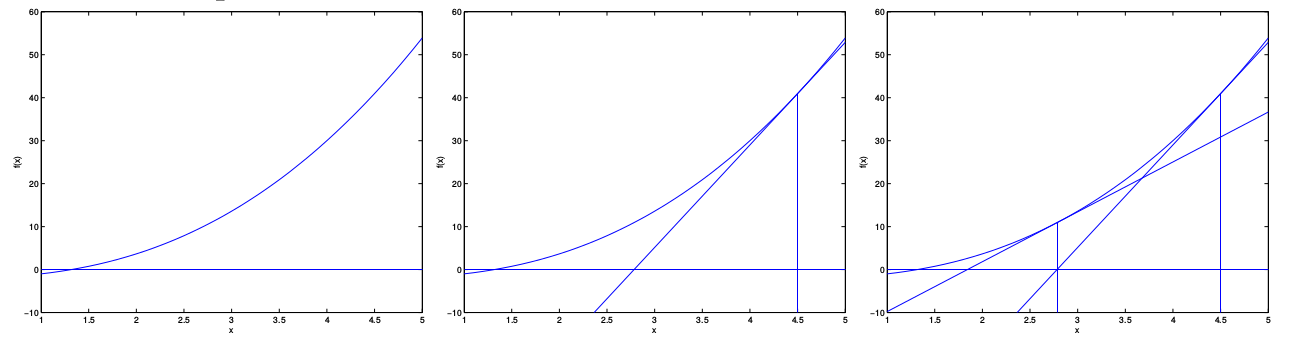
\includegraphics[scale=0.3]{../figures/cs229_2_2.png} 
\end{center}
对于logistic回归的对数似然函数
\begin{eqnarray}
\begin{aligned}
l(\theta) &= \log L(\theta)\\
&= \sum_{i=1}^m y^{(i)}\log h(x^{(i)})+(1-y^{(i)})\log (1-h(x^{(i)}))
\end{aligned}
\end{eqnarray}
考虑其最大值,即对$l(\theta)$的导数$l'(\theta)=0$进行求解,若采用牛顿方法,则有
\begin{eqnarray}
\theta:=\theta-\frac{l'(\theta)}{l''(\theta)}
\end{eqnarray}
若$\theta$为一个向量,则更新法则定义为
\begin{eqnarray}
\theta:=\theta-H^{-1}\nabla_\theta l(\theta)
\end{eqnarray}
其中,$H$为Hessian矩阵,其定义如下
\begin{eqnarray}
\begin{aligned}
H_{ij}&=\frac{\partial^2l(\theta)}{\partial\theta_i\partial\theta_j}\\
&= \frac{\partial}{\partial \theta^{(j)}}\sum_{m=1}^M(h_\theta(x_m)-y_m)x_m^{(n)}\\
&= \sum_{m=1}^M\frac{\partial h_\theta(x_m)x_m^{n}}{\partial \theta^{(j)}}\\
&= \sum_{m=1}^Mx_m^{(n)}\frac{\partial g(\theta^Tx_m)}{\partial \theta^Tx_m}\frac{\partial\theta^Tx_m}{\partial\theta^{(j)}}\\
&= \sum_{m=1}^Mx_m^{(n)}g(\theta^Tx_m)(1-g(\theta^Tx_m))x_m^{(j)}\\
&= \sum_{m=1}^Mx_m^{(n)}h_\theta(x_m)(1-h_\theta(x_m))x_m^{(j)}
\end{aligned}
\end{eqnarray}
因而
\begin{eqnarray}
\begin{aligned}
H&=\nabla_\theta^2l(\theta)\\
&= X^TRX
\end{aligned}
\end{eqnarray}
其中
\begin{eqnarray}
R=
\begin{pmatrix}
h_\theta(x_1)(1-h_\theta(x_1)) & 0 &\cdots & 0\\
0 & h_\theta(x_2)(1-h_\theta(x_2)) & \cdots & 0\\
\vdots & \vdots & \ddots & \vdots\\
0 & 0 & \cdots & h_\theta(x_m)(1-h_\theta(x_m))
\end{pmatrix}
\end{eqnarray}
\section{Fisher线性判别分析}
\subsection{二类线性判别法}
(Fisher)线性判别分析(Linear Discriminant Analysis,简称FDA)是一种经典的线性学习算法。思想是:给定训练样例集,设法将样例投影到一条直线上,使得同类样例的投影点尽量接近,不同类的投影点尽可能远。对于要预测的数据点,投影之后,按位置来划分样本类别。
\begin{center}
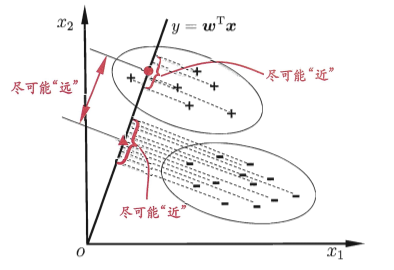
\includegraphics[scale=1]{../figures/LDA1.PNG} 
\end{center}
对于二分类问题,给定数据集$D=\{\sample{x}{i},\sample{y}{i}\}^m_{i=1},y_i\in \{0,1\}$,令$X_i,\mu_i,S_i$分别表示第$i\in\{0,1\}$类的样本的集合、均值向量、协方差矩阵。
\begin{eqnarray}
\mu_i &=& \frac{1}{N_i}\sum_{j\in C_i}\sample{x}{j} = \frac{1}{N_i}\sum_{j=1}^N \sample{x}{j}1(\sample{y}{j}=i)\\
S_i &=& \sum_{j\in C_i}(\sample{x}{j}-\mu_i)(\sample{x}{j}-\mu_i)^T = \sum_{j=1}^N (\sample{x}{j}-\mu_i)(\sample{x}{j}-\mu_i)^T1(\sample{y}{j}=i)
\end{eqnarray}
其中,$C_i$代表第$i\in\{0,1\}$类的样本的集合,$N_i$代表第$i\in\{0,1\}$类的样本个数,$N=N_1+N_2$,$1()$代表示性函数。

若将数据投影到向量$w$(列向量),即$w^Tx$,则第$i$类的均指向量在$w$上的投影为
\begin{eqnarray}
\begin{aligned}
&\ \frac{1}{N_i}\sum_{j\in C_i}w^T\sample{x}{j}\\
&=w^T\frac{1}{N_i}\sum_{j\in C_i}\sample{x}{j}\\
&=w^T\mu_i
\end{aligned}
\end{eqnarray}
第$i$类的协方差在$w$上的投影为
\begin{eqnarray}
\begin{aligned}
&\ \sum_{j\in C_i}(w^T\sample{x}{j}-w^T\mu_i)(w^T\sample{x}{j}-\mu_i)^T\\
&=\sum_{j\in C_i}(w^T(\sample{x}{j}-\mu_i))(w^T(\sample{x}{j}-\mu_i))^T\\
&=\sum_{j\in C_i}w^T(\sample{x}{j}-\mu_i)(\sample{x}{j}-\mu_i)^Tw\\
&=w^T\sum_{j\in C_i}(\sample{x}{j}-\mu_i)(\sample{x}{j}-\mu_i)^Tw\\
&=w^TS_iw
\end{aligned}
\end{eqnarray}
所以$w^T\mu_i$和$w^TS_iw$均为实数。

让类中心距离尽可能大,即$||w^T\mu_0-w^T\mu_1||^2_2$尽可能大,让同类样例投影点协方差尽可能小,即$w^TS_0w+w^TS_1w$尽可能小,则可得到最大化的目标
\begin{eqnarray}
\begin{aligned}
J&=\frac{||w^T\mu_0-w^T\mu_1||^2_2}{w^TS_0w+w^TS_1w}\\
&=\frac{w^T(\mu_0-\mu_1)(\mu_0-\mu_1)^Tw}{w^T(S_0+S_1)w}
\end{aligned}
\end{eqnarray}
定义“类内三度矩阵”(within-class scatter matrix)
\begin{eqnarray}
\begin{aligned}
S_w &=S_0+S_1\\
&=\sum_{i\in C_0}(\sample{x}{i}-\mu_0)(\sample{x}{i}-\mu_0)^T+\sum_{i\in C_1}(\sample{x}{i}-\mu_1)(\sample{x}{i}-\mu_1)^T
\end{aligned}
\end{eqnarray}
定义“类间散度矩阵”(between-class scatter matrix)
\begin{eqnarray}
\begin{aligned}
S_b=(\mu_0-\mu_1)(\mu_0-\mu_1)^T
\end{aligned}
\end{eqnarray}
则有
\begin{eqnarray}
J=\frac{w^TS_bw}{w^TS_ww}
\end{eqnarray}
这是LDA的最大化目标,称为$S_b$与$S_w$的“广义瑞利商”(generalized Rayleigh quotient)。由于分子和分母都是关于$w$的二次项,因此解与$w$的长度无关,只与方向有关。不是一般性,令$w^TS_ww=1$,有
\begin{eqnarray}
\begin{aligned}
&\min_w\ -w^TS_bw\\
&s.t.\ w^TS_ww=1
\end{aligned}
\end{eqnarray}
使用拉格朗日乘子法,有
\begin{eqnarray}
L(w,\lambda)=-w^TS_bw+\lambda(w^TS_ww-1)
\end{eqnarray}
对$w,\lambda$求偏导,有
\begin{eqnarray}
\frac{\partial F}{\partial w}&=&-(S_b+S_b^T)w+\lambda(S_w+S_w^T)w=0\\
\frac{\partial F}{\partial \lambda}&=&1-w^TS_ww=0
\end{eqnarray}
得到
\begin{eqnarray}
S_bw&=&\lambda S_ww\\
w^TS_ww&=&1
\end{eqnarray}
由于$(\mu_0-\mu_1)^Tw$为常数,记$k=(\mu_0-\mu_1)^Tw$,则有
\begin{eqnarray}
S_bw=k(\mu_0-\mu_1)=\lambda S_ww
\end{eqnarray}
可得
\begin{eqnarray}
w=S_w^{-1}\frac{k}{\lambda}(\mu_0-\mu_1)
\end{eqnarray}
由于只需要得到$w$的方向,因而令$\frac{k}{\lambda}=1$,有
\begin{eqnarray}
w=S_w^{-1}(\mu_0-\mu_1)
\end{eqnarray}
对于$S_w^{-1}$的计算,为了数值解的稳定性,通常对$S_w$进行奇异值分解,有
$S_w=U\Sigma V^T$,之后有$S_w^{-1}=V\Sigma^{-1}U^T$。

对于一个新的数据点$x$,计算其投影点分别到$w^T\mu_1$和$w^T\mu_2$的距离,作差,有
\begin{eqnarray}
\begin{aligned}
D&=(w^T\mu_1-w^Tx)^2-(w^T\mu_2-w^Tx)^2\\
&=(w^T\mu_1)^2+(w^Tx)^2-2w^T\mu_1w^Tx-(w^T\mu_2)^2-(w^Tx)^2+2w^T\mu_2w^Tx\\
&=(w^T\mu_1)^2-(w^T\mu_2)^2-2(w^T\mu_1-w^T\mu_2)w^Tx\\
&=(w^T\mu_1+w^T\mu_2)(w^T\mu_1-w^T\mu_2)-2(w^T\mu_1-w^T\mu_2)w^Tx\\
&=(w^T\mu_1-w^T\mu_2)(w^T\mu_1+w^T\mu_2-2w^Tx)\\
&=(w^T\mu_1-w^T\mu_2)(w^T(\mu_1+\mu_2-2x))
\end{aligned}
\end{eqnarray}
当$w^T(\mu_1+\mu_2-2x)>0$时,$D>0$,则$x$判定为第2类;当$w^T(\mu_1+\mu_2-2x)<0$时,$D<0$,则$x$判定为第1类。


\section{分类相关问题}
\subsection{多分类学习}
考虑用二分类学习器来解决多分类的问题。考虑$N$个类别$C_1,C_2,\cdots,C_N$,则将多分类任务拆分为若干个二分类任务求解,测试时,对这些分类器的预测结果进行集成,以获得最终多分类结果。
\subsubsection{一对一策略(One vs One,OvO)}
对给定数据集$D=\{(\sample{x}{1},\sample{y}{1}),(\sample{x}{2},\sample{y}{2}),\cdots,(\sample{x}{m},\sample{y}{m})\},\sample{y}{i}\in\{ C_1,C_2,\cdots,C_N \}$,OvO将$N$个类别两两配对,产生$\frac{N(N-1)}{2}$个二分类任务,其中,分类器把$D$中的$C_i$类样例作为正例,将$C_j$类样例作为反例。测试时,将新样本提交给所有分类器,得到$\frac{N(N-1)}{2}$个分类结果,最终结果通过投票产生。如下图所示
\begin{center}
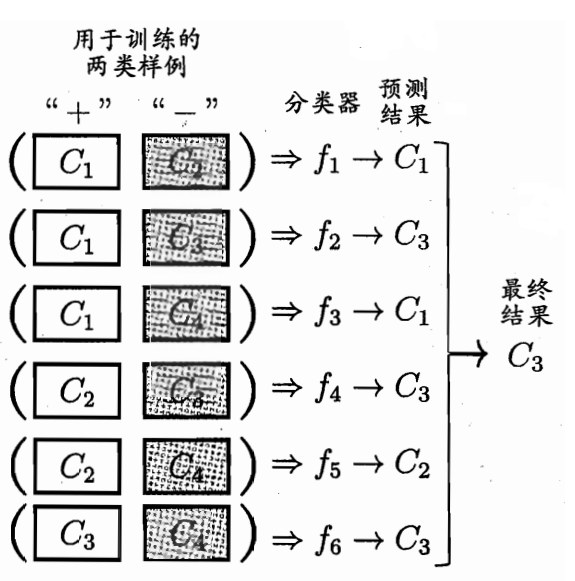
\includegraphics[scale=0.5]{../figures/CP1.PNG} 
\end{center}
可用矩阵来记录这个过程。初始化一个$N\times N$的0矩阵$A$。对于用来训练的两个样例$(C_i,C_j)$,若$C_i$为正例,$C_j$为反例,则记$A_{i,j}=1,A_{j,i}=0$;若$C_i$为反例,$C_j$为正例,则记$A_{i,j}=0,A_{j,i}=1$,如下
\begin{equation}
\begin{pmatrix}
0 & 1 & 0 & 1\\
0 & 0 & 0 & 1\\
1 & 1 & 0 & 1\\
0 & 0 & 0 & 0\\
\end{pmatrix}
\end{equation}
按行求和,可得到$(2,1,3,0)^T$,投票结果为$C_3$最多。则判断为$C_3$。
\subsubsection{一对其余策略(One vs Rest,OvR)}
OvR每次将一个类作为正例,其他类作为反例进行训练,得到$N个$分类器。测试时,若仅有一个分类器预测为正类,则对应的类别标记作为最终的分类结果;若有多个分类器预测为正类,则比较这些分类器的预测置信度,选择置信度最大的。

OvR只需要训练$N$个分类器,而OvO需要训练$\frac{N(N-1)}{2}$个分类器,因而OvO的存储开销和测试时间通常比OvR大,但由于OvO的每个分类器仅用到了两个类的样例,因而OvO的训练时间开销通常比OvR更小。

\subsection{类别不平衡问题}
对于二分类问题,若正例和反例的个数基本相等,对于一个线性分类器$y=f(x)$,则分类器决策规则为
\begin{eqnarray}
\begin{aligned}
\mbox{若}\frac{y}{1-y}>1 , \mbox{则预测为正例}
\end{aligned}
\end{eqnarray}
若正例和反例的个数不等,记$m^+$为正例数目,$m^-$为反例数目,则有
\begin{eqnarray}
\begin{aligned}
\mbox{若}\frac{y}{1-y}>\frac{m^+}{m^-} , \mbox{则预测为正例}
\end{aligned}
\end{eqnarray}
此时则需要对训练集进行调整。
\subsubsection{欠采样(undersampling)}
欠采样法若随机丢弃反例,则可能丢失一些重要的信息,常用的有EasyEnsemble算法。
\paragraph{EasyEnsemble算法}则是利用集成学习的机制,将多数类划分为若干个集合,使得这些多数类的子集中元素个数与少数类样本数量基本相同,供给不同学习器使用,最后将这些学习器集成起来。这样对每个学习器来看都进行了欠采样,但从全局来看,却不会丢失重要的信息。记多数类的样本集合为$L$,少数类样本集合为$S$,$N$为将多数类拆分成$N$个子集来训练$N$个分类器,算法如下
\begin{lstlisting}[language=python]
For i=1,`$\cdots$`,N
   (1) `随机从$L$中抽出样本构成多数类子集$L_1$,使得$|L_i|=|S|$`
   (2) `使用$L_i$和$S$的数据集,训练AdaBoost分类器$F_i$,其中$f_{ij}(x)$为弱分类器`
       `$$F_i(x)=sgn(\sum_{j=1}^n w_{ij}f_{ij}(x)-b_i)$$`
`将上述分类器联合起来`
`$$F(x)=sgn(\sum_{i=1}^N F_i(x))$$`
\end{lstlisting}

\paragraph{balance cascade}

\subsubsection{过采样(oversampling)}
若过采样法简单地对初始样本进行重复采样,很容易引起过拟合。一种方法是SMOTE算法,通过对训练集里的样本进行插值来产生额外的正例。
\paragraph{SMOTE算法}基本思想是根据少数类样本,生成新样本并添加到数据集中,步骤如下
\begin{itemize}
\item[1] 对于少数类$S$中每一个样本$x$,计算其到少数类样本集$S$中所有样本的距离,得到$K$个近邻;
\item[2] 根据样本不平衡比例里设置一个采样比例来确定采样倍率$N$,对于每一个少数类样本$x$,从其$k$近邻中随机选取若干个样本,假设选择的近邻为$\hat{x}$;
\item[3] 对于每一个随机选出的近邻$\hat{x}$,分别与原样本按照如下的公式构建新的样本
\begin{eqnarray}
x_{new}=x + rand(0,1)\times(\hat{x}-x)
\end{eqnarray}
其含义是在$x$和$\hat{x}$所成的线段上任取一个点。
\end{itemize}

该算法主要存在两方面的问题:一是在近邻选择时,存在一定的盲目性。从上面的算法流程可以看出,在算法执行过程中,需要确定$K$值,即选择多少个近邻样本,这需要用户自行解决。从$K$值的定义可以看出,$K$值的下限是$M$值($M$值为从$K$个近邻中随机挑选出的近邻样本的个数,且有$M < K$),$M$的大小可以根据负类样本数量、正类样本数量和数据集最后需要达到的平衡率决定。但K值的上限没有办法确定,只能根据具体的数据集去反复测试。因此如何确定$K$值,才能使算法达到最优这是未知的。 

另外,该算法无法克服非平衡数据集的数据分布问题,容易产生分布边缘化问题。由于负类样本的分布决定了其可选择的近邻,如果一个负类样本处在负类样本集的分布边缘,则由此负类样本和相邻样本产生的“人造”样本也会处在这个边缘,且会越来越边缘化,从而模糊了正类样本和负类样本的边界,而且使边界变得越来越模糊。这种边界模糊性,虽然使数据集的平衡性得到了改善,但加大了分类算法进行分类的难度.

\paragraph{Borderline-SMOTE1}记多数类的样本集合为$L$,少数类样本集合为$S$,$r=\frac{|S|}{|L|}$为少数类与多数类的比例。此算法用来提升SMOTE。步骤如下
\begin{itemize}
\item[1] 对于少数类$S$中每一个样本$x$,计算其到少数类样本集$S$中所有样本的距离,得到$K$个近邻,记该集合为$M_p$。计算样本$x$的这$K$个近邻属于$L$的数量,记为$m'=|M_p\cap L|$
\item[2] 若$m'=m$,则$x$是一个噪声点,不做任何操作;
\item[3] 若$0\leq m'\leq \frac{m}{2}$,说明$x$安全,不做任何操作;
\item[4] 若$\frac{m}{2}\leq m' \leq m$,则说明点$x$危险,需要在这个点附近生成一些新的少数类点,所以将它加入到集合$dange$中;
\item[5] 对于集合$danger$中的点$d$,使用SMOTE算法生成新的样本。
\end{itemize}

Borderline-SMOTE2与Borderline-SMOTE1很像,只是最后一步不一样。全部的步骤如下
\paragraph{Borderline-SMOTE2}记多数类的样本集合为$L$,少数类样本集合为$S$,$r=\frac{|S|}{|L|}$为少数类与多数类的比例。此算法用来提升SMOTE。步骤如下
\begin{itemize}
\item[1] 对于少数类$S$中每一个样本$x$,计算其到少数类样本集$S$中所有样本的距离,得到$K$个近邻,记该集合为$M_p$。计算样本$x$的这$K$个近邻属于$L$的数量,记为$m'=|M_p\cap L|$
\item[2] 若$m'=m$,则$x$是一个噪声点,不做任何操作;
\item[3] 若$0\leq m'\leq \frac{m}{2}$,说明$x$安全,不做任何操作;
\item[4] 若$\frac{m}{2}\leq m' \leq m$,则说明点$x$危险,需要在这个点附近生成一些新的少数类点,所以将它加入到集合$dange$中;
\item[5] 对于集合$danger$中的点$d$,分别在$S$和$L$中得到$k$个最近邻样本$S_k$和$L_k$。在$S_k$中选出$\alpha$比例的样本点和$d$作随机线性插值产生新的少数类样本。在$L_k$中选出$1-\alpha$比例的样本点和$d$做随机的线性插值产生新的少数类样本.
\end{itemize}
\subsubsection{权值移动(threshold-moving)}









\section{指数函数族与广义线性模型}
参数为$\eta$的变量$x$的指数族分布定义为
\begin{eqnarray}
p(x|\eta)=h(x)g(\eta)e^{\eta^Tu(x)}
\end{eqnarray}
其中,$x$可为标量或向量,离散或连续的。
\subsection{伯努利分布导出logistic回归}
考虑伯努利分布,其为二元变量的取值分步。可通过该分布导出logistic函数。伯努利分布及其指数式变形如下
\begin{eqnarray}
\begin{aligned}
p(x|\eta)&=\textbf{Bern}(x|\eta)\\
&=\mu^x(1-\mu)^{1-x}\\
&=e^{x\ln\mu+(1-x)\ln(1-\mu)}\\
&=(1-\mu)e^{\ln(\frac{\mu}{1-\mu})x}
\end{aligned}
\end{eqnarray}
令$h(x)=1$,$g(\eta)=1-\eta$,$\eta^T=\ln(\frac{\mu}{1-\mu})$,$u(x)=x$,因而有
\begin{eqnarray}
\mu=\ln(\frac{\mu}{1-\mu})
\end{eqnarray}
其反函数为
\begin{eqnarray}
\sigma(\eta)=\frac{1}{1+e^{-\eta}}
\end{eqnarray}
因而,logistic回归的形式为
\begin{eqnarray}
y=\sigma(\theta^Tx)
\end{eqnarray}
\subsection{多项式分布导出softmax回归}
考虑多项式分布,其有$M$个可能取值,$\mu_i$为当$x=i$时的概率,因而有
\begin{eqnarray}
\sum_{k=1}^M=1
\end{eqnarray}
定义指示函数
\begin{eqnarray}
I=
\left\lbrace
\begin{aligned}
1,\textbf{True}\\
0,\textbf{False}
\end{aligned}
\right.
\end{eqnarray}
则多项式分布可表示为
\begin{eqnarray}
\begin{aligned}
p(x|\mu) &= \prod_{k=1}^M\mu_k^{I(x_k=1)}\\
&= \exp
	\left\lbrace
	\begin{aligned}
	{\sum_{k=1}^Mx_k\ln\mu_k}\\
	\end{aligned}
	\right\rbrace\\
&= \exp
	\left\lbrace
	\begin{aligned}
	{\sum_{k=1}^{M-1}x_k\ln\mu_k+(1-\sum_{k=1}^{M-1}x_k)\ln(1-\sum_{k=1}^{M-1}\mu_k)}
	\end{aligned}
	\right\rbrace\\
&= \exp
	\left\lbrace
	\begin{aligned}
	\sum_{k=1}^{M-1}x_k\ln(\frac{\mu_k}{1-\sum_{j=1}^{M-1}})+\ln(1-\sum_{k=1}^{M-1}\mu_k)
	\end{aligned}
	\right\rbrace
\end{aligned}
\end{eqnarray}
其为指数族函数,其中
\begin{eqnarray}
\begin{aligned}
h(x)&=1\\
g(\eta)&=1-\sum_{k=1}^{M-1}\mu_k\\
\eta &= 
\begin{pmatrix}
\frac{\mu_1}{1-\sum_{j=1}^{M-1}}\\
\frac{\mu_2}{1-\sum_{j=1}^{M-1}}\\
\vdots\\
\frac{\mu_{M-1}}{1-\sum_{j=1}^{M-1}}
\end{pmatrix}\\
u(x)&=x
\end{aligned}
\end{eqnarray}
令
\begin{eqnarray}
\ln
\left(
\begin{aligned}
\frac{\mu_k}{1-\sum_j\mu_j}
\end{aligned}
\right)
=\eta_k
\end{eqnarray}
求其反函数,有
\begin{eqnarray}
\mu_k=\frac{\exp(\eta_k)}{1+\sum_j^{M-1}\exp(\eta_j)}
\end{eqnarray}
该函数为logistic函数在多元情况下的拓展,称为softmax函数或归一化指数。采用广义线性模型的想法,有
\begin{eqnarray}
p(C_K|x)=y_k=\frac{e^{\theta_k^Tx}}{\sum_je^{\theta_k^Tx}}
\end{eqnarray}
对于第$n$个样本,有
\begin{eqnarray}
\prod_{k=1}^Kp(C_K|x_n)^{I(x_k=1)}=y_k^{I(x_k=1)}
\end{eqnarray}
所以其似然函数为
\begin{eqnarray}
L(\theta)= \prod_{n=1}^N\prod_{k=1}^Kp(C_K|x_n)^{I(x_{nk}=1)}=\prod_{n=1}^N\prod_{k=1}^Ky_{nk}^{I(x_{nk}=1)}
\end{eqnarray}
\section{支持向量机}
在logistic回归中,概率$p(y=1|x;\theta)$由$h_\theta(x)=g(\theta^Tx)$得出。当$h_\theta(x)\geq 0.5$时认为预测值为1,而这种情况对应的是$\theta^Tx\geq0$。当$\theta_Tx$越大,则$p(y=1|x;\theta,b)$则越大,可以认为更加确信预测值是1。因此当有$\theta^Tx\gg0$,认为$y=1$的结果是非常有信心的;相反当有$\theta^Tx\ll0$,认为$y=0$的结果是非常有信心的。因而对于一个训练集,我们或许可以找到一个好的模型,即找到$\theta$,使当$y^{(i)}=1$时,有$\theta^Tx^{(i)}\gg0$,当$y^{(i)}=0$时,有$\theta^Tx^{(i)}\ll0$。事实上,支持向量机(Support Vector Machine)就是采取上述的思想,找到一个分割平面,让训练集的数据点离平面尽可能远。
\subsection{说明}
首先考虑二分类问题,用$y\in\{-1,1\}$而不是$\{0,1\}$来表示类标签;区别于logistic回归中对于线性模型的表示$\theta^Tx$,采用参数$w,b$,则分类器如下
\begin{eqnarray}
h_{w,b}(x)=g(w^Tx+b)\\
g(z)=
\left\lbrace
\begin{aligned}
1&, z\geq 0\\
-1&, otherwise
\end{aligned}
\right.
\end{eqnarray}
在这里,$w,b$的表示法可以截距$b$和其他参数$w$区分出来。于此同时,我们也去掉了$x$中的$x_0=1$这个与$b$相配套的维度。
\subsection{函数间隔与几何间隔}
\subsubsection{函数间隔}
对给定的训练数据$(x^{(i)},y^{(i)})$,定义函数间隔
\begin{eqnarray}
\hat{\gamma}^{(i)}=y^{(i)}(w^Tx+b)
\end{eqnarray}
如果$y^{(i)}=1$,为了让数据点离平面够大,则可让$\hat{\gamma}^{(i)}$足够大,则可让$w^Tx+b\gg0$。相反的,如果$y^{(i)}=-1$,为了让数据点离平面够大,则可让$\hat{\gamma}^{(i)}$足够大,则可让$w^Tx+b\ll0$。因而,可以得到足够大的函数间隔,可以得到置信度高且正确的预测。

然而,函数间隔的一个属性,使得其不能作为一个好的指标来度量置信度(有多大的把握正确):对于给定的$g$,如果用$2w$和$2b$分别代替$w$和$b$,因为$g(w^Tx+b)=g(2w^Tx+2b)$,所以$h_{w,b}(x)=h_{2w,2b}(x)$,然而函数间隔已经改变:
\begin{eqnarray}
2y^{(i)}(w^Tx+b)=y^{(i)}(2w^Tx+2b)
\end{eqnarray}
因此若$w,b$没有限制,则可以让函数间隔任意大,但其实际是没有意义的。因而考虑引入一些像$||w||_2=1$的正则化条件,或者可以用$(\frac{w}{||w||_2},\frac{b}{||w||_2})$来替代原有的$(w,b)$。这些后面会有所提及。

对于给定的训练集$S=\{(x^{(i)},y^{(i)});i=1,\cdots,m\}$,定义训练集$S$的函数间隔为
\begin{eqnarray}
\hat{\gamma}=\min_{i=1,\cdots,m}\hat{\gamma}^{(i)}
\end{eqnarray}
\subsubsection{几何间隔}
考虑下图:
\begin{center}
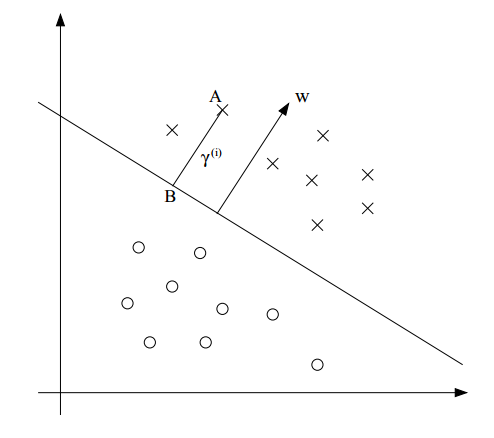
\includegraphics[scale=0.6]{../figures/SVM1.PNG} 
\end{center}
其中,实线为超平面$w^T+b$,向量$w$为超平面的法向量,则$\frac{w}{||w||_2}$位超平面的单位法向量。点$A$表示某个数据点,其所在位置代表输入向量$x^{(i)}$且其标签$y^{(i)}=1$,A到超平面距离为$\gamma^{(i)}$,其为$||AB||_2$。则有
\begin{eqnarray}
\overrightarrow{BA}=\frac{w}{||w||_2}\gamma^{(i)}
\end{eqnarray}
则
\begin{eqnarray}
B=x^{(i)}-\frac{w}{||w||_2}\gamma^{(i)}
\end{eqnarray}
由B在平面上,则有
\begin{eqnarray}
w^T\left( x^{(i)}-\frac{w}{||w||_2}\gamma^{(i)} \right)+b=0
\end{eqnarray}
则可以解出
\begin{eqnarray}
\begin{aligned}
\gamma^{(i)}&=\frac{w^Tx^{(i)}+b}{||w||_2}\\
&=\left(\frac{w}{||w||_2}\right)x^{(i)}+\frac{b}{||w||_2}
\end{aligned}
\end{eqnarray}
因而对于训练集中的数据$(x^{(i)},y^{(i)})$,定义几何间隔
\begin{eqnarray}
\gamma^{(i)}=y^{(i)}
\left(
\left(\frac{w}{||w||_2}
\right)^Tx^{(i)}+\frac{b}{||w||_2}
\right)
\end{eqnarray}
可见,当$||w||_2=1$时,函数间隔等于几何间隔。当用$2w$和$2b$分别代替$w$和$b$时,由于分母$||w||_2$的作用,使得
\begin{eqnarray}
y^{(i)}
\left(
\left(\frac{w}{||w||_2}
\right)^Tx^{(i)}+\frac{b}{||w||_2}
\right)
=
y^{(i)}
\left(
\left(\frac{2w}{||2w||_2}
\right)^Tx^{(i)}+\frac{2b}{||2w||_2}
\right)
\end{eqnarray}
几何间隔保持不变。因而可以对$w,b$进行任意的缩放,让其具有一些独特性质。

对于给定的训练集$S=\{(x^{(i)},y^{(i)});i=1,\cdots,m\}$,定义训练集$S$的几何间隔为
\begin{eqnarray}
\gamma=\min_{i=1,\cdots,m}\gamma^{(i)}
\end{eqnarray}

\subsection{最优间隔分类器}
根据上述方法,为了找到一个超平面将训练集分类,且训练集到超平面的几何间隔最大,有如下公式
\begin{eqnarray}
\begin{aligned}
\max_{\gamma,w,b}\gamma\\
s.t. & \sample{y}{i}(w^T\sample{x}{i}+b)\geq \gamma,i=1,\cdots,m\\
& ||w||=1
\end{aligned}
\end{eqnarray}
对于上述优化问题,由于$||w||=1$非凸,难以用最优化软件求解,因而尝试变型
\begin{eqnarray}
\begin{aligned}
\max_{\gamma,w,b}\frac{\hat{\gamma}}{||w||}\\
s.t. & \sample{y}{i}(w^T\sample{x}{i}+b)\geq \gamma,i=1,\cdots,m\
\end{aligned}
\end{eqnarray}
由于$\frac{\hat{\gamma}}{||w||}$非凸,需要进一步变型。考虑到可以对$w,b$进行缩放,使得$\hat{\gamma}=1$,又求解$\frac{\hat{\gamma}}{||w||}=\frac{\hat{1}}{||w||}$的最大值等价于求解$\frac{1}{2}||w||^2$的最小值,则有
\begin{eqnarray}
\begin{aligned}
\min_{\gamma,w,b} &\ \frac{1}{2}||w||^2\\
s.t. &\ \sample{y}{i}(w^T\sample{x}{i}+b)\geq 1,i=1,\cdots,m\
\end{aligned}
\end{eqnarray}
此时,这个形式的优化问题可以高效求解,其包含凸二次项和线性约束项,这给出了最有间隔分类器。

\subsection{约束优化问题}
\subsubsection{等式约束优化问题}
考虑以下的问题
\begin{eqnarray}
\begin{aligned}
\min_w &\ f(w)\\
s.t. &\ h_i(w)=0,i=1,\cdots,l
\end{aligned}
\end{eqnarray}
定义拉格朗日算子(Lagrangian)如下
\begin{eqnarray}
\mathcal{L}(w,\beta)=f(w)+\sum_{i=1}^l\beta_ih_i(w)
\end{eqnarray}
其中,$\beta_i$称为拉格朗日乘子(Lagrange multipliers),对上式分别对$w_i$和$\beta_i$求偏导
\begin{eqnarray}
\frac{\partial\cal{L}}{\partial w_i}&=&0,i=1,2,\cdots,n\\
\frac{\partial\cal{L}}{\partial \beta_i}&=&0,i=1,2,\cdots,l\\
\end{eqnarray}
从而求解q$w$和$\beta$。得到的解可能极值点,此方程组称为等式约束的极值必要条件。此方法相当于将拉格朗日乘子$\beta_i$和$x_i$一起看为优化变量,则优化变量个数增加为$n+l$个。$\beta_i$和$x_i$一视同仁,均为优化变量,均对他们求偏导。

\subsubsection{不等式约束优化问题}
考虑一个一元函数的例子
\begin{eqnarray}
\begin{aligned}
\min &\ f(x)\\
s.t. &\ g_1(x)=a-x\leq 0\\
&\ g_2(x)=x-b\leq 0
\end{aligned}
\end{eqnarray}

对于约束$g_1$和$g_2$,我们分别引入两个松弛变量$a_1^2$和$b_1^2$,得到$$h_1(x,a_1)=g_1+a_1^2=0$和$h_2(x,b_1)=g_2+b_1^2=0$,此处考虑加上平方项$a_1^2,b_1^2$而不是$a_1,b_1$,因为其能隐含的反映其大于等于0的性质。若只加上$a_1$和$b_1$,则需要引入新的约束$a_1\geq 0$和$b_1\geq 0$,这会让问题复杂化。于是,我们将不等式约束转化为了等式约束
\begin{eqnarray}
\begin{aligned}
\min &\ f(x)\\
s.t. &\ h_1(x,a_1)=g_1+a_1^2=a-x+a_1^2=0\\
&\ h_2(x,b_1)=g_2+b_1^2=x-b+b_1^2=0
\end{aligned}
\end{eqnarray}
于是可以得到拉格朗日函数
\begin{eqnarray}
\mathcal{L}(x,a_1,b_1,\mu_1,\mu_2)=f(x)+\mu_1(a-x+a_1^2)+\mu_2(x-b+b_1^2)
\end{eqnarray}
对各变量求偏导,联立方程,有
\begin{eqnarray}
\left\lbrace
\begin{aligned}
\frac{\partial \mathcal{L}}{\partial x}=\frac{\partial f}{\partial x}+\mu_1\frac{dg_1}{dx}+\mu_2\frac{dg_2}{dx}=\frac{df}{dx}-\mu_1+\mu_2=0,\\
\frac{\partial \mathcal{L}}{\partial \mu_1}=g_1+a_1^2=0,\ \frac{\partial \mathcal{L}}{\partial \mu_2}=g_2+b_1^2=0,\\
\frac{\partial \mathcal{L}}{\partial a_1}=2\mu_1a_1=0,\ 
\frac{\partial \mathcal{L}}{\partial b_1}=2\mu_2b_1=0,\\
\mu_1\geq 0,\ \mu_2\geq 0
\end{aligned}
\right.
\end{eqnarray}
其可转化为
\begin{eqnarray}
\left\lbrace
\begin{aligned}
\frac{\partial f}{\partial x}+\mu_1\frac{dg_1}{dx}+\mu_2\frac{dg_2}{dx}=0,\\
\mu_1g_1=0,\ \mu_2g_2=0,\\
\mu_1\geq 0,\ \mu_2\geq 0
\end{aligned}
\right.
\end{eqnarray}
对于多元多次不等式约束问题
\begin{eqnarray}
\begin{aligned}
\min_w &\ f(x)\\
s.t.&\  g_j(x)\leq0(j=1,2,\cdots,m)
\end{aligned}
\end{eqnarray}
有
\begin{eqnarray}
\left\lbrace
\begin{aligned}
\frac{\partial f(x^*)}{\partial x_i}+\sum_{j=1}^m\mu_j\frac{\partial g_j(x^*)}{\partial x_i}=0, i=1,2\cdots,n,\\
\mu_jg_j(x^*)=0, j=1,2,\cdots,m,\\
\mu_j\geq 0,j=1,2,\cdots,m
\end{aligned}
\right.
\end{eqnarray}
上式称为不等式约束优化问题的KKT(Karush-Kuhn-Tucker)条件,$\mu_j$称为KKT乘子。当约束起作用时$\mu_j> 0,g_j(x)=0$,约束不起作用时有$\mu_j= 0,g_j(x)<0$。\footnote{参考自https://zhuanlan.zhihu.com/p/26514613}

让其与CS229采用同样的记法,对于原问题
\begin{eqnarray}
\begin{aligned}
\min_w &\ f(w)\\
s.t. &\ g_i(w)\leq0,i=1,\cdots,k\\
&\ h_i(w)=0,i=1,\cdots,l
\end{aligned}
\end{eqnarray}
拉格朗日函数为
\begin{eqnarray}
\mathcal{L}(w,\alpha,\beta)=f(w)+\sum_{i=1}^k\alpha_ig_i(w)+\sum_{i=1}^l\beta_ih_i(w)
\end{eqnarray}
考虑量
\begin{eqnarray}
\theta_p(w)&=&\max_{\alpha,\beta:\alpha\geq0}\mathcal{L}(w,\alpha,\beta)\\
&=&\max_{\alpha,\beta:\alpha\geq0}\ f(w)+\sum_{i=1}^k\alpha_ig_i(w)+\sum_{i=1}^l\beta_ih_i(w)
\end{eqnarray}
定义原问题的最优值为
\begin{eqnarray}
p^*=\min_w\theta_p(w)
\end{eqnarray}
另一方面,考虑对偶问题,可得到
\begin{eqnarray}
\theta_D(\alpha,\beta)=\min_w\mathcal{L}(w,\alpha,\beta)
\end{eqnarray}
定义对偶问题的最优值为
\begin{eqnarray}
d^*=\max_{\alpha,\beta:\beta_i\geq0}\theta_D(w)
\end{eqnarray}
原问题和对偶问题的关系为
\begin{eqnarray}
d^*=\max_{\alpha,\beta:\beta_i\geq0}\min_w\mathcal{L}(w,\alpha,\beta)\leq \min_w\max_{\alpha,\beta:\beta_i\geq0}\mathcal{L}(w,\alpha,\beta)=p^*
\end{eqnarray}
当
\begin{eqnarray}
d^*=p^*
\end{eqnarray}
时,为强对偶,此时,原问题和对偶问题会取相同的值。\\

所得的KKT条件为
\begin{eqnarray}
\frac{\partial}{\partial w_i}\mathcal{L}(w^*,\alpha^*,\beta^*)&=&0,i=1,\cdots,n\\
\frac{\partial}{\partial \beta_i}\mathcal{L}(w^*,\alpha^*,\beta^*)&=&0,i=1,\cdots,l\\
\alpha_i^*g_i(w^*)&=&0,i=1,\cdots,k\\
g_i(w^*)&\leq&0,i=1,\cdots,k\\
\alpha^*&\geq& 0,i=1,\cdots,k
\end{eqnarray}
如果$w^*,\alpha^*,\beta^*$满足KKT条件,则其为原问题和对偶问题的一个解。其中,$\alpha_i^*g_i(w^*)=0,i=1,\cdots,k$被称为KKT对偶互补条件( KKT dual complementarity condition),它表明如果$\alpha_i^*>0$,则$g_i(w^*)=0$
\subsection{最优间隔分类器的求解}
对之前,已得到
\begin{eqnarray}
\begin{aligned}
\min_{\gamma,w,b} &\ \frac{1}{2}||w||^2\\
s.t. &\ \sample{y}{i}(w^T\sample{x}{i}+b)\geq 1,i=1,\cdots,m\
\end{aligned}
\end{eqnarray}
可将约束写成
\begin{eqnarray}
g_i(w)=-\sample{y}{i}(w^T\sample{x}{i}+b)+1\leq 0,
\end{eqnarray}
从KKT对偶互补条件可知,当训练数据点的函数间隔等于1时,才会有$\alpha_i>0$
其拉格朗日函数为
\begin{eqnarray}
\mathcal{L}(w,b,\alpha)=\frac{1}{2}||w||^2-\sum_{i=1}^m\alpha_i\sample{y}{i}(w^T\sample{x}{i}+b)-1]
\end{eqnarray}
其中,$\alpha_i$为KKT乘子,而不需要$\beta_i$拉格朗日乘子,因为该问题中只有不等式约束。

考虑下图:

\begin{center}
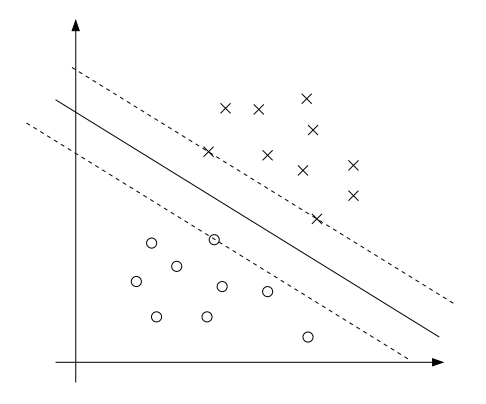
\includegraphics[scale=0.6]{../figures/SVM2.PNG} 
\end{center}
其中,实线表示最大间隔平面。图中,有三个点的间隔最小,有一个是负类,两个是正类,它们位于与超平面平行的虚线上。因此,这三个数据点所对应的$\alpha_i$非0,我们称这三个数据点为该问题的支持向量(support vectors)。事实上,支持向量的数目会比训练集中的数据数目少很多。

解对偶问题,首先固定$\alpha$,对$\mathcal{L}(w,b,\alpha)$,分别求$w,b$的偏导,令偏导数等于0,有
\begin{eqnarray}
\nabla_w\mathcal{L}(w,b,\alpha)=w-\sum_{i=1}^m\alpha_i\sample{y}{i}\sample{x}{i}&=&0\\
\frac{\partial}{\partial b}\mathcal{L}(w,b,\alpha)&=&0
\end{eqnarray}
得
\begin{eqnarray}
w&=&\sum_{i=1}^m\alpha_i\sample{y}{i}\sample{x}{i}\\
\sum_{i=1}^m\alpha_i\sample{y}{i}&=&0
\end{eqnarray}
代入则有
\begin{eqnarray}
\begin{aligned}
\mathcal{L}(w,b,\alpha)&=\frac{1}{2}w^Tw-\sum_{i=1}^m\alpha_i(\sample{y}{i}(w^T\sample{x}{i}+b)-1)\\
&=\frac{1}{2}\left(\sum_{i=1}^m \alpha_i\sample{y}{i}\sample{x}{i}\right)^T\left(\sum_{i=j}^m \alpha_j\sample{y}{j}\sample{x}{j}\right)-
\sum_{i=1}^m\alpha_i
	( 
	\sample{y}{i} 
		(
			(
				\left(\sum_{i=j}^m \alpha_j\sample{y}{j}\sample{x}{j}\right)^T\sample{x}{i}+b
			)-1
		) 
	)\\
&=\frac{1}{2}\sum_{i=1}^m\sum_{j=1}^m\sample{y}{i}\sample{y}{j}\alpha_i\alpha_j\langle\sample{x}{i},\sample{x}{j}\rangle-\sum_{i=1}^m\sum_{j=1}^m\sample{y}{i}\sample{y}{j}\alpha_i\alpha_j\langle\sample{x}{i},\sample{x}{j}\rangle+\sum_{i=1}^m\alpha_i\\
&=\sum_{i=1}^m\alpha_i-\frac{1}{2}\sum_{i=1}^m\sum_{j=1}^m\sample{y}{i}\sample{y}{j}\alpha_i\alpha_j\langle\sample{x}{i},\sample{x}{j}\rangle-b\sum_{i=1}^m\alpha_i\sample{y}{i}\\
&=\sum_{i=1}^m\alpha_i-\frac{1}{2}\sum_{i=1}^m\sum_{j=1}^m\sample{y}{i}\sample{y}{j}\alpha_i\alpha_j\langle\sample{x}{i},\sample{x}{j}\rangle
\end{aligned}
\end{eqnarray}
其中,$\langle\sample{x}{i},\sample{x}{j}\rangle=(\sample{x}{i})^T\sample{x}{j}$,令
\begin{eqnarray}
W(\alpha)=\sum_{i=1}^m\alpha_i-\frac{1}{2}\sum_{i=1}^m\sum_{j=1}^m\sample{y}{i}\sample{y}{j}\alpha_i\alpha_j\langle\sample{x}{i},\sample{x}{j}\rangle
\end{eqnarray}
我们可以得到如下的原问题的对偶问题
\begin{eqnarray}
\begin{aligned}
\max_\alpha&\ W(\alpha)=\sum_{i=1}^m\alpha_i-\frac{1}{2}\sum_{i=1}^m\sum_{j=1}^m\sample{y}{i}\sample{y}{j}\alpha_i\alpha_j\langle\sample{x}{i},\sample{x}{j}\rangle\\
s.t.&\ \alpha_i\geq 0,i=1,2,\cdots,m\\
&\ \sum_{i=1}^m\alpha_i\sample{y}{i}=0
\end{aligned}
\end{eqnarray}
其符合KKT条件,因而可以求解$\alpha$,通过$w=\sum_{i=1}^m\alpha_i\sample{y}{i}\sample{x}{i}$求解$w$,对于$b$的求解,考虑到可以用离超平面最相近的两类点的中点来求$b$。设上面求得的$w$为$w^*$,则有
\begin{eqnarray}
b^*=-\frac{\max_{i:\sample{y}{i}=-1}w^{*T}\sample{x}{i}+\min_{i:\sample{y}{i}=1}w^{*T}\sample{x}{i}}{2}
\end{eqnarray}

\subsection{核方法}
定义原始输入值为某个问题的输入属性(input attributes),由输入属性延伸出来的新变量定义为输入特征(input features),用$\phi$表示特征映射,比如如下的将输入属性映射为输入特征的函数
\begin{eqnarray}
\phi(x)=
\begin{pmatrix}
x\\
x^2\\
x^3
\end{pmatrix}
\end{eqnarray}

由于我们可以得到的最优间隔分类器为如下形式
\begin{eqnarray}
\begin{aligned}
\max_\alpha&\ W(\alpha)=\sum_{i=1}^m\alpha_i-\frac{1}{2}\sum_{i=1}^m\sum_{j=1}^m\sample{y}{i}\sample{y}{j}\alpha_i\alpha_j\langle\sample{x}{i},\sample{x}{j}\rangle\\
s.t.&\ \alpha_i\geq 0,i=1,2,\cdots,m\\
&\ \sum_{i=1}^m\alpha_i\sample{y}{i}=0
\end{aligned}
\end{eqnarray}
对于算法中所含有$\langle x,z\rangle$,我们可以将其替换为$\langle\phi(x),\phi(z)\rangle$。另外,对于给定的特征映射$\phi$,定义其对应的核(kernel)为
\begin{eqnarray}
K(x,z)=\phi(x)^T\phi(z)
\end{eqnarray}
因此,对于算法中含有的$\langle x,z\rangle$,我们可以替换为$K(x,z)$,此时算法就可以基于特征函数$\phi$来学习。

对于给定的$\phi$,我们可以通过计算$\phi(x)$和$\phi(z)$以及计算其内积来很容易地得到$K(x,z)$。虽然$K(x,z)$计算的代价不高,但$\phi(x)$计算代价可能会很高(可能因为它是一个非常高维的向量)。在这种设置下,我们让SVMs在更高维度中学习(对于给定的$\phi$),而不需要显式地调用向量$\phi(x)$

考察土哥例子。对于$x,z\in \mathbb{R}^n$,考虑
\begin{eqnarray}
\begin{aligned}
K(x,z)&=(x^Tz)^2\\
&= \left(\sum_{i=1}^nx_iz_i\right)\left(\sum_{j=1}^nx_jz_j\right)\\
&= \sum_{i=1}^n\sum_{j=1}^nx_ix_jz_iz_j\\
&= \sum_{i=1}^n\sum_{j=1}^n(x_ix_j)(z_iz_j)
\end{aligned}
\end{eqnarray}
因此,$K(x,z)=\phi(x)^T\phi(z)$,其中特征映射$\phi$为如下形式(只给出$n=3$时的情况)
\begin{eqnarray}
\phi(x)=
\begin{pmatrix}
x_1x_1\\
x_1x_2\\
x_1x_3\\
x_2x_1\\
x_2x_2\\
x_2x_3\\
x_3x_1\\
x_3x_2\\
x_3x_3
\end{pmatrix}
\end{eqnarray}
这种情况下,计算高维的$\phi(x)$需要$O(n^2)$的时间,而$K(x,z)$只需要$O(n)$的时间。

作为一个相似的核,考虑
\begin{eqnarray}
\begin{aligned}
K(x,z)&=(x^Tz+c)^2\\
&=\left(\sum_{i=1}^nx_iz_i+c\right)\left(\sum_{j=1}^nx_jz_j+c\right)\\
&=\sum_{i=1}^n\sum_{j=1}^n(x_ix_j)(z_iz_j)+2c\sum_{i=1}^nx_iz_i+c^2\\
&=\sum_{i=1}^n\sum_{j=1}^n(x_ix_j)(z_iz_j)+\sum_{i=1}^n(\sqrt{2c}x_i)(\sqrt{2c}z_i)+c^2
\end{aligned}
\end{eqnarray}
则其相应的特征映射为
\begin{eqnarray}
\phi(x)=
\begin{pmatrix}
x_1x_1\\
x_1x_2\\
x_1x_3\\
x_2x_1\\
x_2x_2\\
x_2x_3\\
x_3x_1\\
x_3x_2\\
x_3x_3\\
\sqrt{2c}x_1\\
\sqrt{2c}x_2\\
\sqrt{2c}x_3\\
c
\end{pmatrix}
\end{eqnarray}
其中,参数$c$用来控制$x_i$和$x_ix_j$的权重。

更一般的,核$K(x,z)=(x^Tz+c)^d$对应一个特征映射(映射到$\left(_d^{n+d}\right)$的特征空间)。虽然是在$O(n^d)$维空间中计算,但是计算$K(x,z)$依然只需要$O(n)$的时间,因此,我们不需要显式地在很高维的特征空间中表示特征向量。

接下来,考察一种略微不同的核。直观地,若$\phi(x)$和$\phi(z)$非常接近,则我们希望$K(x,z)=\phi(x)T\phi(z)$是大的。相反的,若$\phi(x)$和$\phi(z)$距离很远(假设已经接近彼此正交),则我们希望$K(x,z)=\phi(x)T\phi(z)$是小的。因此设想$K(x,z)$是一种度量规则,来度量$\phi(x)$和$\phi(z)$有多接近,或者$x$和$z$有多接近。

\subsubsection{高斯核函数}
直觉上,可能会想到这样的一个函数
\begin{eqnarray}
K(x,z)=\exp\left(
-\frac{||x-z||^2}{2\sigma^2}
\right)
\end{eqnarray}
当$x$和$z$接近时,则该值趋近与1;当距离远时,该值趋近于0。它可以用作SVM的一个核。(这个核称为高斯核,对应于有限维特征映射$\phi$)。

\subsubsection{核的有效性}
作为问题的推广,对于给定的函数$K$,如何判断其是否是有效的核?比方说有这样的问题:是否存在特征映射$\phi$,使对于所有$x,z$,都有$K(x,z)=\phi(x)^T\phi(z)$?

假设$K$确实是一个对应于某个特征映射$\phi$的有效的核,那么考虑有限的$m$个点的集合$\{\sample{x}{1},\cdots,\sample{x}{m}\}$,定义一个$m\times m$的方阵$K$,其中$K_{ij}=K(\sample{x}{i},\sample{x}{j})$,并将$K$称为核矩阵(Kernel matrix)。

若$K$是一个有效的核,则
\begin{eqnarray}
\begin{aligned}
K_{ij} &= K(\sample{x}{i},\sample{x}{j})\\
&= \phi(\sample{x}{i})^T\phi(\sample{x}{j})\\
&= \phi(\sample{x}{j})^T\phi(\sample{x}{i})\\
&= K(\sample{x}{j},\sample{x}{i})\\
&= K_{ji}
\end{aligned}
\end{eqnarray}
因此,$K$必须是对称的。定义$\phi_k(x)$为向量$\phi(x)$的第$k$个维度,则对于任意的向量$z$,我们有
\begin{eqnarray}
\begin{aligned}
z^TKz&=\vectornew{z}{m}\matrixthird{K}{m}{m}\vvectornew{z}{m}\\
&= \left(\sum_{i=1}^mZ_iK_{i1},\sum_{i=1}^mZ_iK_{i2},\cdots,\sum_{i=1}^mZ_iK_{im}\right)\vvectornew{z}{m}\\
&= \sum_i^m\sum_j^mz_iK_{ij}z_j\\
&= \sum_i^m\sum_j^mz_i\phi(\sample{x}{i})^T\phi(\sample{x}{j})z_j\\
&= \sum_i^m\sum_j^mz_i\sum_k^m\phi_k(\sample{x}{i})\phi_k(\sample{x}{j})z_j\\
&= \sum_k^m\sum_i^m\sum_j^mz_i\phi_k(\sample{x}{i})\phi_k(\sample{x}{j})z_j\\
&= \sum_k^m\left(\sum_{i=1}z_i\phi_k(\sample{x}{i})\right)\\
&\geq 0
\end{aligned}
\end{eqnarray}
由于$z^TKz\geq 0$,且$z$是任意的,因为$K$是半正定矩阵($K\geq 0$)。

因此,如果$K$是一个有效的核(设其对应于特征映射$\phi$),那么其对应的核矩阵$K\in \mathbb{R}^{m\times m}$是半正定的。这是充分非必要的。这个有效的核称为Mercer kernel。

\paragraph{Mercer 定理} $K$是$\mathbb{R}^n\times\mathbb{R}^n\mapsto\mathbb{R}$的映射,$K$是有效的(kercer)核的充分必要条件为对于任意$\{\sample{x}{1},\cdots,\sample{x}{m}\}$,$m<\infty$,其对应的核矩阵是半正定的。

其中,任意$\{\sample{x}{1},\cdots,\sample{x}{m}\}$是任意一个包含有$m$个样本的集合,并不一定是训练集,可以任选。

对于给定的函数$K$,除了尝试找到一个对应于$K$的特征映射$\phi$,该理论给出了另一种方法去测试$K$是否是一个有效核。


\subsection{正则化和非线性可分情况}
到目前SVM假设数据是线性可分的。因为通过$\phi$将数据映射到高维的特征空可以提高数据可分的可能性,但是我们不能保证一直可以达到这种效果。而且有的时候我们也不必赢定要去寻找这个超平面,由于一些异常点。举个例子,左边表示了一个最优的间隔分类器,但当一个异常点加入到了左边的数据点之后,导致判平面发生了戏剧性的旋转,而且其产生的分类器只有一个很小的间隔。
\begin{center}
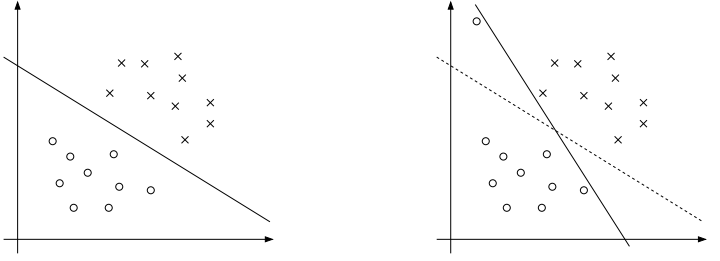
\includegraphics[scale=0.6]{../figures/SVM3.PNG} 
\end{center}

为了让算法适用于非线性可分的数据,同时降低对于异常点的灵敏性,我们重新修改了最优化分类器,其结果如下
\begin{eqnarray}
\begin{aligned}
\min_{\gamma,w,b}&\ \frac{1}{2}||w||^2+C\sum_{i=1}^m\xi_i\\
s.t.&\ \sample{y}{i}(w^T\sample{x}{i}+b)\geq 1-\xi_i,i=1,\cdots,m\\
&\ \xi_i\geq 0,i=1,\cdots,m
\end{aligned}
\end{eqnarray}
因此,这种改进可以允许函数间隔小于1,若有某个例子的函数间隔为$1-\xi_i$,它将会在目标函数上付出$C\xi_i$的代价。参数$C$用来权衡要让$||w||^2$大(将会让函数间隔变小)还是尽量保证大部分的数据能够有函数间隔至少等于1。

就像之前的,我们可以得到拉格朗日函数如下
\begin{eqnarray}
\mathcal{L}(w,b,\xi,\alpha,r)=\frac{1}{2}||w||^2+C\sum_{i=1}^m\xi_i-\sum_{i=1}^m\alpha_i[\sample{y}{i}(w^T\sample{x}{i}+b)-1+\xi_i]-\sum_{i=1}^mr_i\xi_i
\end{eqnarray}

其中,$\alpha_i$和$r_i$是KKT乘子。分别对$w,b,\xi$求偏导,有
\begin{eqnarray}
\nabla_w\mathcal{L}=w-\sum_{i=1}^m\alpha_i\sample{y}{i}\sample{x}{i}=0\\
\nabla_n\mathcal{L}=-\sum_{i=1}^m\alpha_i\sample{y}{i}=0\\
\nabla_{\xi_i}\mathcal{L}=C-\alpha_i-r_i=0,i=1,2,\cdots,m
\end{eqnarray}

\begin{eqnarray}
\begin{aligned}
\mathcal{L}(w,b,\xi,\alpha,r)&=\frac{1}{2}||w||^2+C\sum_{i=1}^m\xi_i-\sum_{i=1}^m\alpha_i[\sample{y}{i}(w^T\sample{x}{i}+b)-1+\xi_i]-\sum_{i=1}^mr_i\xi_i\\
&=\frac{1}{2}w^Tw+C\sum_{i=1}^m\xi_i-\sum_{i=1}^m\alpha_i[\sample{y}{i}(w^T\sample{x}{i}+b)-1+\xi_i]-\sum_{i=1}^mr_i\xi_i\\
&=\frac{1}{2}w^Tw-\sum_{i=1}^m\alpha_i[\sample{y}{i}(w^T\sample{x}{i}+b)-1]+C\sum_{i=1}^m\xi_i-\sum_{i=1}^m\alpha_i\xi_i-\sum_{i=1}^mr_i\xi_i\\
&=\frac{1}{2}w^Tw-\sum_{i=1}^m\alpha_i[\sample{y}{i}(w^T\sample{x}{i}+b)-1]+
\begin{pmatrix}
C\\
C\\
\vdots\\
C
\end{pmatrix}^T\vvectornew{\xi}{m}-\vvectornew{\alpha}{m}^T\vvectornew{\xi}{m}-\vvectornew{r}{m}^T\vvectornew{\xi}{m}\\
&=\frac{1}{2}w^Tw-\sum_{i=1}^m\alpha_i[\sample{y}{i}(w^T\sample{x}{i}+b)-1]+
\begin{pmatrix}
C-\alpha_1-r_1\\
C-\alpha_2-r_2\\
\vdots\\
C-\alpha_m-r_m
\end{pmatrix}^T\vvectornew{\xi}{m}\\
&=\frac{1}{2}w^Tw-\sum_{i=1}^m\alpha_i[\sample{y}{i}(w^T\sample{x}{i}+b)-1]\\
&=\sum_{i=1}^m\alpha_i-\frac{1}{2}\sum_{i=1}^m\sum_{j=1}^m\sample{y}{i}\sample{y}{j}\alpha_i\alpha_j\langle\sample{x}{i},\sample{x}{j}\rangle
\end{aligned}
\end{eqnarray}

我们可以得到如下的原问题的对偶问题
\begin{eqnarray}
\begin{aligned}
\max_\alpha&\ W(\alpha)=\sum_{i=1}^m\alpha_i-\frac{1}{2}\sum_{i=1}^m\sum_{j=1}^m\sample{y}{i}\sample{y}{j}\alpha_i\alpha_j\langle\sample{x}{i},\sample{x}{j}\rangle\\
s.t.&\ 0\leq \alpha_i \leq C,i=1,2,\cdots,m\\
&\ \sum_{i=1}^m\alpha_i\sample{y}{i}=0
\end{aligned}
\end{eqnarray}

就像之前一样,$w$依旧可以通过$\alpha$表示。让我们震惊的是,增加了$\mathcal{l}_1$正则项,对偶问题的改变只是在原有基础上由$0\leq\alpha_i$变为$0\leq\alpha_i\leq C$,$b^*$的求解也与之前一样。

同样的,KKT对偶互补条件(这些将在SMO算法中用到)如下
\begin{eqnarray}
\alpha_i=0 \Rightarrow \sample{y}{i}(w^T\sample{x}{i}+b)\geq 1\\
\alpha_i=C \Rightarrow \sample{y}{i}(w^T\sample{x}{i}+b)\leq 1\\
0<\alpha_i<C \Rightarrow \sample{y}{i}(w^T\sample{x}{i}+b)=1
\end{eqnarray}

\subsection{SMO算法}
SMO算法( sequential minimal optimization algorithm)给出一种有效率的方法来解决SVM所引出的对偶问题。首先考虑坐标提升算法(coordinate ascent algorithm)。

\subsubsection{坐标提升}
考虑解决一个无约束最优化问题
\begin{eqnarray}
\max_\alpha\ W\vectornew{\alpha}{m}
\end{eqnarray}
这里,我们认为$W$是一个关于$\alpha_i$的函数,而且我们先忽略任何该问题与SVMs的关系。接下来我们要探讨一个新的优化算法,称为梯度提升法:

\begin{center}
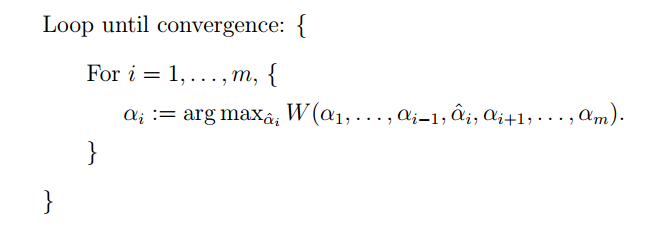
\includegraphics[scale=1]{../figures/SVM4.PNG} 
\end{center}

在算法的最里层循环中,我们让除了$\alpha_i$以外的变量保持固定,然后通过调整参数$\alpha_i$来反复优化$W$。在该算法的表示中,里层循环根据次序$\alpha_1,\alpha_2,\cdots,\alpha_m,\alpha_1,\alpha_2,\cdots$来反复优化变量。(其他更加复杂的版本可能会选择其他的次序,比如,我们可能会选择能够最大增长$W(\alpha)$的变量来优化。)

当函数$W$采取$\arg\max$的方式,则坐标提升将很有效率。下图为坐标提升的图
\begin{center}
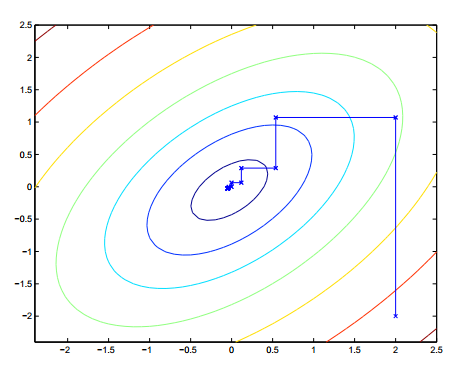
\includegraphics[scale=1]{../figures/SVM5.PNG} 
\end{center}

其中,椭圆表示我们要优化的二次函数的等高线。从坐标$(-2,2)$开始坐标提升,在图中画出其收敛到全局最大值的路径。可以注意到坐标提升每一步迭代都是平行于坐标轴,因一次为只有一个变量呗最优化。

\subsubsection{SMO}
下面的对偶优化问题我们将要求解的:
\begin{eqnarray}
\begin{aligned}
\max_\alpha&\ W(\alpha)=\sum_{i=1}^m\alpha_i-\frac{1}{2}\sum_{i=1}^m\sum_{j=1}^m\sample{y}{i}\sample{y}{j}\alpha_i\alpha_j\langle\sample{x}{i},\sample{x}{j}\rangle\\
s.t.&\ 0\leq \alpha_i \leq C,i=1,2,\cdots,m\\
&\ \sum_{i=1}^m\alpha_i\sample{y}{i}=0
\end{aligned}
\end{eqnarray}
假设我们有满足约束条件的$\alpha_i$的集合。现在,我们保持$\alpha_2,\cdots,\alpha_m$不变,然后用坐标提升的方法,通过优化$\alpha_1$来优化目标函数。但是这个方法是不可行的,因为约束条件有
\begin{eqnarray}
\alpha_1\sample{y}{1}=-\sum_{i=2}^m\alpha_i\sample{y}{i}
\end{eqnarray}
由于$\sample{y}{i}\in\{-1,1\}$,则有$(\sample{y}{1})^2=1$。对上式两边同时乘$\sample{y}{1}$,则可以得到
\begin{eqnarray}
\begin{aligned}
\alpha_1&=\alpha_1(\sample{y}{1})^2=-\sample{y}{1}\sum_{i=2}^m\alpha_i\sample{y}{i}
\end{aligned}
\end{eqnarray}
因此,$\alpha_1$由其他的$\alpha_i,i\neq1$确定。如果我们保持$\alpha_2,\cdots,\alpha_m$不变,则$\alpha_1$不能变,除非我们违背约束条件。因此,如果我们想要更新其中一些$\alpha$,则我们至少要同时改变两个以满足约束条件。于是其催生了SMO算法,其工作原理如下:
\begin{center}
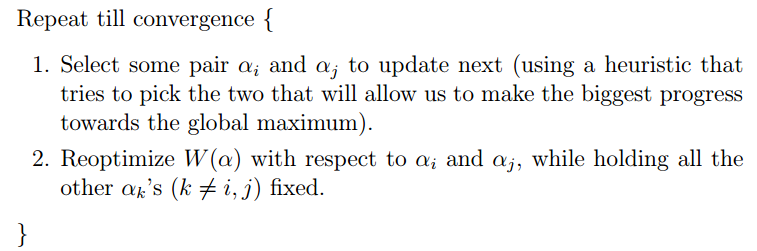
\includegraphics[scale=1]{../figures/SVM6.PNG} 
\end{center}
对于验证算法何时收敛,我们检验如下的KKT对偶互补条件是否在$tol$中,$tol$代表convergence tolerance parameter,其经常被设置在0.01到0.001。
\begin{eqnarray}
\alpha_i=0 \Rightarrow \sample{y}{i}(w^T\sample{x}{i}+b)\geq 1\\
\alpha_i=C \Rightarrow \sample{y}{i}(w^T\sample{x}{i}+b)\leq 1\\
0<\alpha_i<C \Rightarrow \sample{y}{i}(w^T\sample{x}{i}+b)=1
\end{eqnarray}
SMO是高效的算法的主要原因是$\alpha_i$和$\alpha_j$的更新是容易计算出来的。假设我们有满足约束条件的$\alpha$的取值集合,然后我们保持$\alpha_3,\cdots,\alpha_m$不变,然后通过优化$\alpha_1$和$\alpha_2$来优化$W(\alpha_1,\alpha_2,\cdots,\alpha_m)$。通过式
\begin{eqnarray}
\sum_{i=1}^m\alpha_i\sample{y}{i}=0
\end{eqnarray}
我们可以得到
\begin{eqnarray}
\alpha_1\sample{y}{1}+\alpha_2\sample{y}{2}=-\sum_{i=3}^m\alpha_i\sample{y}{i}
\end{eqnarray}
由于等号右边是固定的,我们假设是常数$\zeta$,则有
\begin{eqnarray}
\alpha_1\sample{y}{1}+\alpha_2\sample{y}{2}=\zeta
\end{eqnarray}
则我们可以得到如下图像
\begin{center}
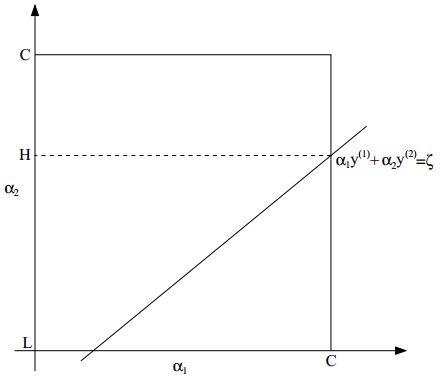
\includegraphics[scale=1]{../figures/SVM7.PNG} 
\end{center}
由约束$0\leq\alpha_i\leq C,i=1,\cdots,m$,我们可知$\alpha_1$和$\alpha_2$必须被限制在$[0,C]\times[0,C]$的框中。直线为$\alpha_1\sample{y}{1}+\alpha_2\sample{y}{2}=\zeta$。从以上的约束可以看出$L\leq\alpha_2\leq H$,否则$(\alpha_1,\alpha_2)$无法同时满足在框中的约束和直线上的约束。

又由于
\begin{eqnarray}
\alpha_1=(\zeta-\alpha_2\sample{y}{2})\sample{y}{1}
\end{eqnarray}
因此我们可以把$W(\alpha)$写成如下的形式
\begin{eqnarray}
W(\alpha_1,\alpha_2,\cdots,\alpha_m)=W((\zeta-\alpha_2\sample{y}{2})\sample{y}{1},\alpha_2,\cdots,\alpha_m)
\end{eqnarray}
将$\alpha_3,\cdots,\alpha_m$看做是常量,我们可以将$W$看作是$\alpha_2$的二次函数。如果我们忽视框的约束,那么很容易通过对二次函数求导令其等于0来求得。我们用$\alpha_2^{new,unclipped}$来表示$\alpha_2$的结果。如果我们通过最大化$W$求得的$\alpha_2$在框的约束之外,那么我们可以在$\alpha_2^{new,unclipped}$的基础上进行修剪,让其落于$[L,H]$之间,于是可以得到如下结果
\begin{eqnarray}
\alpha_2^{new}=
\left\lbrace
\begin{aligned}
H,&\ \ if \alpha_2^{new,unclipped}>H\\
\alpha_2^{new,unclipped}&\ \ if L\leq \alpha_2^{new,unclipped} \leq H\\
L,&\ \ if \alpha_2^{new,unclipped}<L
\end{aligned}
\right.
\end{eqnarray}
最后,找到了$\alpha_2^{new}$之后,再求$\alpha_1^{new}$即可。





\section{学习理论}
\subsection{偏差与方差的权衡}
当在谈及线性回归时,我们在探讨应该用类似$y=\theta_0+\theta_1x$“简单”的模型还是用多项式$y=\theta_0+\theta_1x+\cdots+\theta_x^5$的“复杂”的模型来拟合。我们可以看到如下例子
\begin{center}
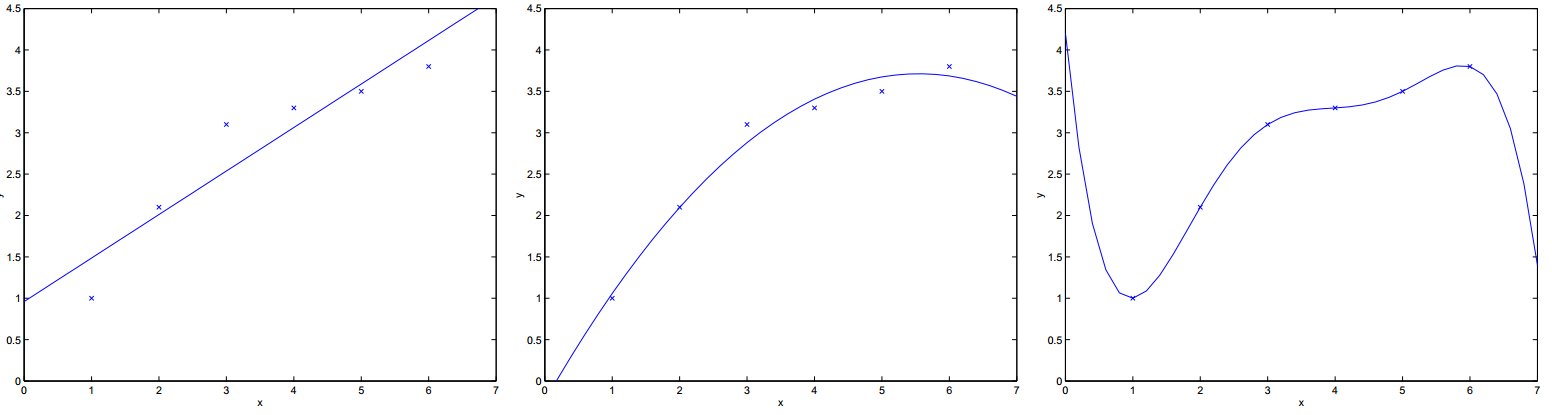
\includegraphics[scale=0.5]{../figures/LT1.PNG} 
\end{center}
拟合5次多项式曲线不是一个好的模型。特殊的,即使是五次的多项式能够很好地从$x$预测$y$,我们还是不认为这个模型十号的。换句话说,这个模型对其他的数据的一般化并不好。我们定义一个假设的泛化误差(generalization error)为该假设的期望风险(error),样本不止来源于训练集。

从上图可以看出,左边的和右边的模型都有较大的泛化误差。然而,这两个模型所遭遇的问题不一样。若$y$与$x$的关系不是线性的,则即使我们有大量的数据,用线性模型去提取数据的特征也会失败。非正式的,我们定义一个模型的偏差(bias)为期望泛化误差。因此,对上面的问题,线性模型有较大的偏差,对于数据可能是欠拟合的情况。

除了偏差,第二个泛化误差的成分为模型拟合的偏差(variance)。特殊的,当像右边的图一样拟合一个五次多项式曲线时,有很大的风险是我们现在提取的数据特征刚好是符合现有的小规模的有限数据集,但是对更大规模的数据并不适用。

因此,经常性的,偏差和方差有权衡。若模型很“简单”,而且具有很少的参数,则其可能会有较大的偏差(但是方差是小的);若模型很“复杂”,而且具有很多的参数,则其可能会有较大的方差(但是偏差是小的)。在以上的例子中,拟合一个二次曲线会比一次曲线和五次曲线这些极端条件要好。

\subsection{引入}
接下来的引理将对下文有所帮助。我们也尝试去探究一些问题:
\begin{itemize}
\item 我们是否可以解决偏差和方差的权衡?
\item 在机器学习中,我们关心泛化误差,但是大部分的算法是根据训练集来训练模型的,为什么我们可以通过训练集来获得关于泛化误差的一些信息呢?特殊的,我们能不能得到训练集的误差和泛化误差的关系?
\item 需要继续什么条件,我们才能证明这个学习算法是好的。
\end{itemize}

\paragraph{引理\ 联合界}假设$A_1,A_2,\cdots,A_k$为$k$个不同的事件,则有
\begin{eqnarray}
P(A_1\cup\cdots\cup A_k)\leq P(A_1)+\cdots+P(A_k)
\end{eqnarray}
在概率理论中,联合界作为公理。

\paragraph{引理\ Hoeffding不等式}假设$Z_1,Z_2,\cdots,Z_m$是$m$个独立同分布(independent and identically distributed(iid))的服从伯努利分布$Bernoulli(\phi)$随机变量,即$P(Z_i=1)=\phi$,$P(Z_i=0)=1-\phi$。$\hat{\phi}$为随机变量的均值,即$\hat{\phi}=\frac{1}{m}\sum_{i=1}^mZ_i$,令$\gamma>0$固定,则有
\begin{eqnarray}
P(|\phi-\hat{\phi}|>\gamma)\leq 2e^{-2\gamma^2m}
\end{eqnarray}
这个引理在学习理论中也被称为Chernoff bound。该引理说明,若用$\hat{\phi}$来估计$\phi$,当$m$增大时,估计值与实际值的距离大于$\gamma$的概率将会被减小。

采用这两个引理,我们可以证明一些比较深层且重要的学习理论结论。

为了简化阐述,我们将目光放在二分类问题,其中标签$y\in\{0,1\}$。假设对于给定的训练集$S=\{(\sample{x}{i},\sample{y}{i});i=1,\cdots,m\}$,其规模为$m$,训练样本$(\sample{x}{i},\sample{y}{i})$服从iid的概率分布$\mathcal{D}$。对于假说$h$,定义训练误差(training error)(在学习理论中也称为经验风险(empirical risk )或经验误差(empirical error )),为如下公式:
\begin{eqnarray}
\hat{\epsilon}(h)=\frac{1}{m}\sum_{i=1}^m1\{h(\sample{x}{i})\neq\sample{y}{i}\}
\end{eqnarray}
可知,只有小部分的$h$的分类错误的数据被使用。对于训练集$S$时记为$\hat{\epsilon}_S(h)$。定义泛化误差(generalization error )为
\begin{eqnarray}
\epsilon(h)=P_{(x,y)\sim D}(h(x)\neq y)
\end{eqnarray}
其表明对于新的服从分布$\mathcal{D}$的数据$(x,y)$,其误分类的概率。

我们假设将要用来估计假说的数据是抽取自同一分布$\mathcal{D}$的,这有时也被作为概率近似正确(PAC(probably approximately correct))的一个设想。

设想一个线性分类,让$h_\theta(x)=1\{\theta^Tx\geq0\}$,一种调节参数$\theta$的方式是最小化训练误差,然后选择
\begin{eqnarray}
\hat{\theta}=\arg\min_\theta\hat{\epsilon}(h_\theta)
\end{eqnarray}
我们将这种方法称为经验风险最小化(ERM(empirical risk minimization )),算法的结果为$\hat{h}=h_{\hat{\theta}}$。我们将ERM看作最“基础”的算法。

为了简化讨论,我们定义假设类(hypothesis class)$\mathcal{H}$为以一种学习算法为基础的所有分类器。比如线性回归,则$\mathcal{H}=\{h_\theta:h_\theta=1\{\theta^Tx\geq 0\},\theta\in \mathbb{R}^{n+1}\}$是所有基于$\mathcal{X}$(输入域)的,判定边界为线性的分类器。

于是ERM可以视为如下式子
\begin{eqnarray}
\hat{h}=\arg\min_{h\in\mathcal{H}}\hat{\epsilon}(h)
\end{eqnarray}

\subsection{有限假设类$\mathcal{H}$的情况}
对于一类学习问题,我们定义假设类$\mathcal{H}=\{h_1,\cdots,h_k\}$,包含了$k$种假设。因此,$\mathcal{H}$为包含有$k$个从$\mathcal{X}$映射到$\{0,1\}$的方程的集合。ERM根据这$k$个方程中训练误差最小来选择$\hat{h}$。

接下来准备考察$\hat{h}$的泛化误差,策略分为两步:
\begin{itemize}
\item 说明对于所有$h$,$\hat{\epsilon}(h)$是$\epsilon(h)$的可靠的估计
\item 说明其中应用了$\hat{h}$的泛化误差的上界
\end{itemize}

任选一个$h_i\in \mathcal{H}$并固定。考虑一个伯努利随机变量$Z$,对于采样$(x,y)\in \mathcal{•}cal{D}$,为$Z=1\{h_i(x)\neq y\}$。类似的,我们定义$Z_j=1\{h_i(\sample{x}{j})\neq\sample{y}{j}\}$。$Z$,$Z_j$对$\mathcal{D}$服从独立同分布。

对于随机的样本的误分类概率,$\epsilon(h)$为$Z$和$Z_j$的期望值。同时,训练误差如下
\begin{eqnarray}
\hat{\epsilon}(h_i)=\frac{1}{m}\sum_{j=1}^mZ_j
\end{eqnarray}
其中,$\hat{\epsilon}(h_i)$为$m$个随机变量$Z_j$的均值,其中,$Z_j$服从均值为$\epsilon(h_i)$的独立同分布的伯努利分布。因此,我们可以应用Hoeffding不等式,得到
\begin{eqnarray}
P(|\epsilon(h_i)-\hat{\epsilon}(h_i)|>\gamma)\leq 2e^{-2\gamma^2m}
\end{eqnarray}

这表明,对于特定的$h_i$,当$m$够大时,训练误差将会很高概率地靠近泛化误差。我们将要证明,这个结论在所有的$h\in\mathcal{H}$同时也成立。令事件$A_i$代表$|\epsilon(h_i)-\hat{\epsilon}(h_i)|>\gamma$。其有性质$P(A_i)\leq 2e^{-2\gamma^2m} $,应用联合界定理,我们求在$\mathcal{H}$中存在$h$,使得$|\epsilon(h_i)-\hat{\epsilon}(h_i)|>\gamma$成立的概率
\begin{eqnarray}
\begin{aligned}
P(\exists h\in \mathcal{H}.|\epsilon(h_i)-\hat{\epsilon}(h_i)|>\gamma ) &= P(A_1\cup\cdots\cup A_k)\\
&\leq \sum_{i=1}^kP(A_i)\\
&\leq \sum_{i=1}^k 2e^{-2\gamma^2m}\\
&= 2ke^{-2\gamma^2m}
\end{aligned}
\end{eqnarray}
求其对立事件,有
\begin{eqnarray}
\begin{aligned}
P(\urcorner(\exists h\in \mathcal{H}.|\epsilon(h_i)-\hat{\epsilon}(h_i)|>\gamma)) &= P(\forall h\in \mathcal{H}.|\epsilon(h_i)-\hat{\epsilon}(h_i)|\leq\gamma )
&\geq 1-2ke^{-2\gamma^2m}
\end{aligned}
\end{eqnarray}

其中,$\urcorner$代表“非”。从上可知,对于所有的$h\in\mathcal{H}$,$\epsilon(h)$和$\hat{\epsilon}(h)$的距离小于$\gamma$的概率至少为$1-2ke^{-2\gamma^2m}$。这被称为一致收敛(uniform convergence),因为这个边界同时适用于所有的$h\in\mathcal{H}$。

记$\delta=2ke^{-2\gamma^2m}$,则对于给定的$\gamma$和$\delta>0$,当$m$取多大时,可以保证概率至少有$1-\delta$,使$\epsilon(h)$和$\hat{\epsilon}(h)$的距离小于$\gamma$?我们可以得到
\begin{eqnarray}
2ke^{-2\gamma^2m} \geq \delta \Rightarrow\ m\geq \frac{1}{2\gamma^2}\log\frac{2k}{\delta}
\end{eqnarray}
其中$\log$又为$\ln$。于是就得到了概率至少为$1-\delta$,对于任意的$h\in\mathcal{H}$,有$|\epsilon(h)-\hat{\epsilon}(h)|\leq \gamma$。这就告诉了我们应该需要多少的训练数据来确保这个界。用来确保算法达到一定的性能的数据大小$m$也被称为算法的样本复杂度(sample complexity)。

上面的界限也有一个重要的结论:样本数据的大小和假设数量$k$为对数关系。

类似的,我们可以固定$m$和$\gamma$,然后求解$\gamma$,对于所有的$h\in\mathcal{H}$,我们可以得到
\begin{eqnarray}
|\hat{\epsilon}(h)-\epsilon(h)|\leq \gamma \leq \sqrt{\frac{1}{2m}\log\frac{2k}{\delta}}
\end{eqnarray}

假定$h^*=\arg\min_{h\in\mathcal{H}}\epsilon(h)$为$\mathcal{H}$中最优的假设,我们有
\begin{eqnarray}
\begin{aligned}
\epsilon(\hat{h})&\leq \hat{\epsilon}(\hat{h})+\gamma\\
&\leq \hat{\epsilon}(h^*)+\gamma\\
&\leq \epsilon(h^*)+2\gamma
\end{aligned}
\end{eqnarray}
对于第一行,是应用了$|\epsilon(\hat{h})-\hat{\epsilon}(\hat{h})|\leq \gamma$。第二行是应用了$\hat{h}=\arg\min_{h\in\mathcal{H}}\hat{\epsilon}(h)$,则有$\hat{\epsilon}(\hat{h})\leq \hat{\epsilon}(h)$都成立,则对于特定的$h^*$,也有$\hat{\epsilon}(\hat{h})\leq \hat{\epsilon}(h^*)$成立。第三行则是再次应用了$|\epsilon(\hat{h})-\hat{\epsilon}(\hat{h})|\leq \gamma$,并将$h^*$代入。于是我们可以得到,当一致收敛性成立,则$\hat{h}$的泛化误差与$\mathcal{H}$中最优的假设的泛化误差只会差$2\gamma$。于是可以得到下面的定理

\paragraph{定理}让$|\mathcal{H}|=k$,令$m,\delta$固定,当训练误差和泛化误差的距离小于一定值的概率至少为$1-\delta$时,我们有
\begin{eqnarray}
\epsilon(\hat{h})\leq \left( \min_{h\in\mathcal{H}}\epsilon(h) \right)+2\sqrt{\frac{1}{2m}\log\frac{2k}{\delta}}
\end{eqnarray}

这证明了当$\gamma=\sqrt{\frac{1}{2m}\log\frac{2k}{\delta}}$,一致收敛性成立的概率至少为$1-\delta$,而且一致收敛性由表明了$\epsilon(h)$最多比$\epsilon(h^*)=\min_{h\in\mathcal{H}}\epsilon(h)$高$2\gamma$。

这也为我们在模型选择中的误差(bias)/方差(variance)权衡中提供了量化。特殊的,假设有一个假设类$\mathcal{H}$,另外假设比$\mathcal{H}'$大很多的假设类,且有$\mathcal{H}'\supseteq\mathcal{H}$。当在$\mathcal{H}'$上考虑问题是,则第一项$\min_{h\in\mathcal{H}}\epsilon(h)$会进一步减小。因此,应用了更大的假设类,则误差(bias)只能减小。然而,若$k$增大,则第二项$2\sqrt{\frac{1}{2m}\log\frac{2k}{\delta}}$将会增大,这对应着当应用更大的假设类时方差(variance)会增大。

像前面所做的,固定$\gamma$和$\delta$,求解$m$,我们可以得到样本复杂度界
\paragraph{推论}让$|\mathcal{H}|=k$,令$\gamma,\delta$固定,为了让$\epsilon(\hat{h})\leq \min_{h\in\mathcal{H}}\epsilon(h)+2\gamma$推出训练误差和泛化误差的距离小于$\gamma$的概率至少为$1-\delta$,需要
\begin{eqnarray}
\begin{aligned}
m&\geq \frac{1}{2\gamma^2}\log\frac{2k}{\delta}\\
&=O\left( \frac{1}{\gamma^2}\log\frac{k}{\delta} \right)
\end{aligned}
\end{eqnarray}

\subsection{无限假设类$\mathcal{H}$的情况}
我们已经得到了关于有限假设类的一些结论。但有很多的假设类,包含了所有的数字(像线性回归),实际上包含了无穷的数字,我们可以得到类似的结论吗?

假设$\mathcal{H}$有$d$个实参数。由于我们用计算机来代表实数,而且双精度是使用64位来代表浮点数,所以假设我们的算法是使用双精度的,于是参数为$64d$位。因此,我们的假设类最多有$k=2^{64d}$种不同的假设。从上一节的推论,为了保证$\epsilon(\hat{h})\leq\epsilon(h^*)+2\gamma$来保证概率至少有$1-\delta$,其需要$m\geq O(\frac{1}{\gamma^2}\log\frac{2^{64d}}{\delta})=O(\frac{d}{\gamma^2}\log\frac{1}{\delta})=O_{\gamma,\delta}(d)$,所以训练集大小最多只与模型的参数数量成线性关系。

事实上我们是依赖了64位精度的条件,这不完全符合所要探讨的条件,但是其结论是大致上正确的。如果我们为了最小化训练误差,为了让含有$d$个参数的假设训练地好,则我们需要和$d$成线性条件的训练数据。

\subsubsection{VC维}
给定假设类$\mathcal{H}$和示例集$D=\{\sample{x}{1},\sample{x}{2},\cdots,\sample{x}{d}\}$,$\mathcal{H}$中每个假设$h$都能对$D$中示例赋予标记,标记结果可表示为
\begin{eqnarray}
h|_D=\{ (h(\sample{x}{1}),h(\sample{x}{2}),\cdots,h(\sample{x}{d}) \}
\end{eqnarray}
随着$d$的增加,$\mathcal{H}$种所有假设对$D$种的示例所能赋予标记的可能结果数也会增大

\paragraph{定义\ 增长函数}对所有$d\in\mathbb{N}$,假设空间$\mathcal{H}$的增长函数$\prod_H(d)$为
\begin{eqnarray}
\prod_\mathcal{H}(m)=\max_{\{ \sample{x}{1},\cdots,\sample{x}{d} \}\subseteq\mathcal{X}}|\{ (h(\sample{x}{1}),h(\sample{x}{2}),\cdots,h(\sample{x}{d})|h\in\mathcal{H} \}|
\end{eqnarray}
增长函数$\prod_\mathcal{H}(m)$表示假设类$\mathcal{H}$对$m$个示例所能赋予标记的最大可能结果数。$\mathcal{H}$对示例所能赋予标记的可能结果数越大,$\mathcal{H}$的表示能力越强,对学习任务的适应能力也越强。因此,增长函数描述了假设空间$\mathcal{H}$的表示能力,由此反映出假设空间的复杂度,我们可利用增长函数来估计经验误差与泛化误差之间的关系

\paragraph{定理}对假设类$\mathcal{H}$,$m\in\mathbb{N}$,$0<\epsilon<1$和任意$h\in\mathcal{H}$,有
\begin{eqnarray}
P(|E(h)-\hat{E}(h)|>\epsilon)\leq 4\prod_\mathcal{H}(2m)e^{-\frac{m\epsilon^2}{8}}
\end{eqnarray}

$\mathcal{H}$中的不同假设对于$D$中示例赋予的结果可能相同,也可能不同。尽管$\mathcal{H}$可能包含无穷多种假设,但其对$D$种示例赋予标记可能结果数是有限的。在一个二分类问题中,最多有$2^m$种结果。$\mathcal{H}$中的假设对$D$中示例赋予标记的每种可能结果称为对$D$的一种“对分”。若假设空间$\mathcal{H}$能实现示例集$D$上的所有对分,即$\prod_\mathcal{H}=2^m$,则称示例集$D$能被假设类$\mathcal{H}$“打散”。

\paragraph{定义\ VC维}假设类$\mathcal{H}$的VC维是能被$\mathcal{H}$打散的最大示例集的大小,即
\begin{eqnarray}
VC(\mathcal{H})=\max\{ m:\prod_\mathcal{H}(m)=2^m \}
\end{eqnarray}
$VC(\mathcal{H})=d$表明存在大小为$d$的示例集能被假设类$\mathcal{H}$打散。若$\mathcal{H}$能打散任意大小的集合,则$VC(\mathcal{H})=\infty$。若存在大小为$d$的示例集能被$\mathcal{H}$打散,但不存在任何大小为$d+1$的示例集能被$\mathcal{H}$打散,则$\mathcal{H}$的VC维是$d$。这就意味着不是多有大小为$d$的示例集都能被假设类$\mathcal{H}$打散,VC维的定义与数据分布$\mathcal{D}$无关。因此,在数据分布未知时仍能计算出假设类$\mathcal{H}$的VC维。

对于下图的数据,我们可以用二分类线性分类器$(h(x)=1\{\theta_0+\theta_1 x_1+\theta_2 x_2\})$所组成的假设类$\mathcal{H}$来打散,为以下八种情况
\begin{center}
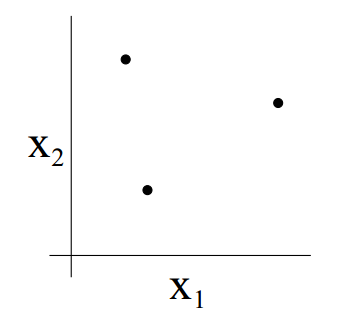
\includegraphics[scale=0.8]{../figures/LT2.PNG} \\
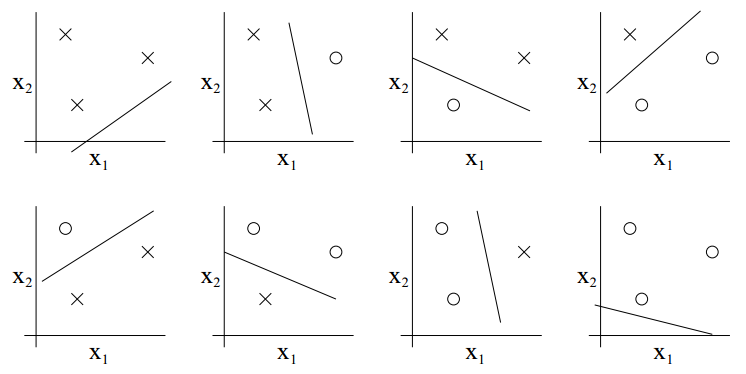
\includegraphics[scale=1]{../figures/LT3.PNG}
\end{center}
由于找不到任何可以被假设类$\mathcal{H}$打散的4个点的数据集,所以$VC(\mathcal{H})=3$。虽然是这样,但有一些三个点的数据是没办法被打散的,比如如下的例子
\begin{center}
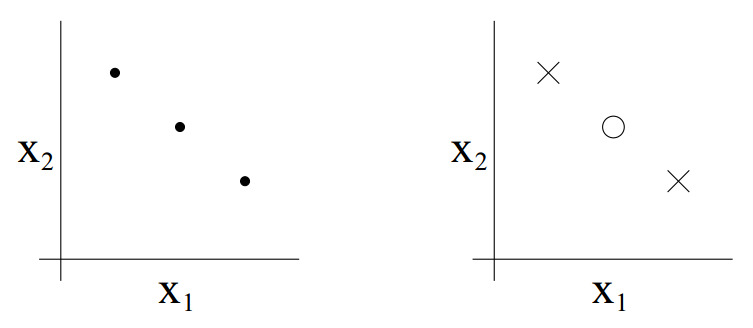
\includegraphics[scale=0.8]{../figures/LT4.PNG}
\end{center}

\paragraph{定理}对于给定的$\mathcal{H}$,且$d=VC(\mathcal{H})$,则为了概率至少能达到$1-\delta$,对于所有的$h\in\mathcal{H}$,有
\begin{eqnarray}
|\epsilon(h)-\hat{\epsilon}(h)|\leq O\left( \sqrt{\frac{d}{m}\log\frac{m}{d}+\frac{1}{m}\log\frac{1}{\delta}}   \right)
\end{eqnarray}
由于概率至少为$1-\delta$,有
\begin{eqnarray}
\epsilon(\hat{h})\leq \epsilon(h^*)+O\left( \sqrt{\frac{d}{m}\log\frac{m}{d}+\frac{1}{m}\log\frac{1}{\delta}}   \right)
\end{eqnarray}
其表明,若一个假设类有有限的VC维,则当$m$增大时,其将一致收敛。于是我们可以得到如下推论

\paragraph{推论}为了$|\epsilon(h)-\hat{\epsilon}(h)|\leq \gamma$来使任意$\in\mathcal{H}$都有概率至少为$1-\delta$,其需要$m=O_{\gamma,\delta}(d)$

这表明,为了让模型能很好的学习,训练集数量需要和$VC(\mathcal{H})$成线性关系。又由于VC维和模型的参数数量成大致的线性关系,因此我们可以得到,训练集所需数量和$\mathcal{H}$的参数数量是成大致的线性关系的。
















\section{正则化与模型选择}
假设我们为了一个学习问题而在多个不同的模型之间做选择。比如,我们要用到多项式回归模型$h_\theta(x)=g(\theta_0,\theta_1x+\cdots,+\theta_kx_k)$,想要确定$k$是应该取$0,\cdots,10$种的一个。我们应该如何自动的选择模型,使其对偏差和方差有好的权衡?

假设我们有有限个模型$\mathcal{M}=\{M_1,\cdots,M_d\}$,我们尝试在其中选取。比如,在上面的模型中,模型$M_i$则表示$i$次的多项式回归模型。如果我们想在SVM,神经网络和逻辑斯蒂回归中选一个,则$\mathcal{M}$是包含这些模型的。

\subsection{交叉验证}
对于给定的训练集$S$,下面的想法是基于ERM的模型选择
\begin{enumerate}[1]
\item 在$S$上训练每个模型$M_i$,得到假设$h_i$
\item 选择有最小训练误差的假设
\end{enumerate}

这个算法不可行,考虑多项式模型,多项式次数越高,则其拟合训练集$S$的效果越好(训练误差越小),因此这种方法倾向于选择高方差的高次的多项式模型。
\subsubsection{留出交叉验证}
下面的方法有所改进。采用留出交叉验证法(hold-out cross validation)(或称为简单交叉验证(simple cross validation)),如下
\begin{enumerate}[1]
\item 随机地将$S$分割成$S_{train}$($70\%$的数据)和$S_{cv}$($30\%$的数据),$S_{cv}$被称为留出交叉验证数据集
\item 用$S_{train}$训练每一个模型$M_i$,得到假设$h_i$
\item 选择在留出交叉验证数据集上误差$\hat{\epsilon}S_{cv}(h_i)$上最小的假设$h_i$。其中,$\hat{\epsilon}S_{cv}(h_i)$指$h$在$S_{cv}$上的训练误差。
\end{enumerate}
一般情况下,留出交叉验证数据集选择数据的$\frac{1}{4}\sim\frac{1}{3}$,$30\%$是通常的选择。事实上,对于第三步,可以修改为在选出了$M_i$之后,再用完整的训练集$S$去训练。

\subsubsection{k折交叉验证}
留出交叉验证法的一个缺点是会“浪费”$30\%$的数据,即使我们有利用这部分数据对所选出来的$M_i$进行再训练,但是只是用了$70\%$的数据来,于是就有如下的算法:k折交叉验证(k-fold cross validation)
\begin{enumerate}[1]
\item 将数据集$S$分割成$k$个不想交的子集,每个子集包含$\frac{k}{m}$个数据,将其记为$S_i,i=1,2,\cdots,k$
\item for $j=1,\cdots,k$\\
\indent\ \ 在数据集$S_1\cup\cdots\cup S_{j-1}\cup S_{j+1}\cup\cdots\cup S_k$得到假设$h_{ij}$,并计算$h_{ij}$在$S_j$上的误差$\hat{\epsilon}_{S_j}(h_{ij})$\\
\indent\ \ 对$\hat{\epsilon}_{S_j}(h_{ij})$在$j$上求均值,得到模型$M_i$上的泛化误差估计值。
\item 选择具有最小的泛化误差模型$M_i$,然后用完整的数据集$S$来重新训练$M_i$。
\end{enumerate}
一种典型的选择是将$k$设为10,虽然数据的比率变为了$\frac{1}{k}$,比以前少很多,而且计算的复杂度也比留出交叉验证要大,因为需要对每个模型训练$k$次。
\subsubsection{留一交叉验证}
当数据量很匮乏时,可能会使用极端的方法:$k=m$。在这种情况下,模型将会在$m-1$的数据集中做训练,用剩下的一个数据做测试。最后也是通过对得到的$m$个模型做平均,得到模型的泛化误差估计值。这种模型称为留一交叉验证(leave-one-out cross validation)。

\subsubsection{自助法}
留一法受训练样本规模变化的影响较小,但计算复杂度又太高,一种方法在减少训练样本规模造成的影响,同时还能比较高效地进行实验估计。

“自助法”(bootstrapping)如下。给定包含$m$个样本的数据集$D$,我们对它进行采样产生数据集$D'$:每次随机从$D$中挑选一个样本,并将其拷贝如$D'$,然后将该样本放回初始数据集$D$中,使这个样本在下一次采样时还可能被采到,这个过程重复执行$m$次后,就得到了包含$m$个样本的数据集$D'$。$D$中有一部分样本会在$D'$中多次出现,而另一部分样本不出现。样本在$m$次采样中始终不被采到的概率时$(1=\frac{1}{m})^m$,取极限有
\begin{eqnarray}
\lim_{m\rightarrow\infty}\left( 1-\frac{1}{m} \right)^m=\frac{1}{e}\sim 0.368
\end{eqnarray}
即通过自主采样,初始数据集$D$中约有$36.8\%$的样本未出现在采样数据集$D'$中,因此可以将$D'$用作训练集,$D-D'$用作测试集。这样,实际评估的模型与期望评估的模型都使用了$m$个训练样本,而仍有数据总量约为$\frac{1}{3}$的没在训练集中出现的样本用于测试。这样的测试结果,称为“包外估计”(out-of-bag estimate)。

自助法在数据集较小、难以有效划分训练集和测试集时很有用,又自助法能从初始数据集中产生多个不同的训练集,这对集成学习等方法有很大的好处。然而,自助法产生的数据集改变了初始数据集的分布,这会引入估计误差。因而,当初始数据量足够时,其他交叉验证法更为常用。

\subsection{性能度量}
性能度量是衡量模型泛化能力的评价标准。在预测任务中,给定样例集$D=\{(\sample{x}{i},\sample{y}{1}),\cdots,(\sample{x}{m},\sample{y}{m})\}$,其中$\sample{y}{i}$是示例$\sample{x}{i}$的真实标记,要评估学习器$f$的性能,就要把学习器预测结果$f(x)$和真实标记$y$进行比较。 
\subsubsection{错误率与精度}
定义分类错误率为
\begin{eqnarray}
E(f;D)=\frac{1}{m}\sum_{i=1}^m 1(f(\sample{x}{i})\neq \sample{y}{i})
\end{eqnarray}
精度定义为
\begin{eqnarray}
acc(f;D)&=&\frac{1}{m}\sum_{i=1}^m 1(f(\sample{x}{i})= \sample{y}{i})\\
&=&1-E(f;D)
\end{eqnarray}
或对于数据分布$\mathcal{D}$和概率密度函数$p(x)$
\begin{eqnarray}
E(f;D)=\int_{x\sim D} 1(f(x)\neq y)p(x)dx
\end{eqnarray}
\begin{eqnarray}
acc(f;D)&=&\int_{x\sim D} 1(f(x)= y)p(x)dx\\
&=&1-E(f;D)
\end{eqnarray}
\subsubsection{查准率、查全率与F1}
对于二分类问题,将真实类别和预测类别的组合分为真正例(true positive),假正例(false positive),真反例(ture negative),假反例(false negative),分别记为$TP,FP,TN,FN$,显然有$TP+FP+TN+FN=$样例总数,定义混淆矩阵如下

\begin{center}
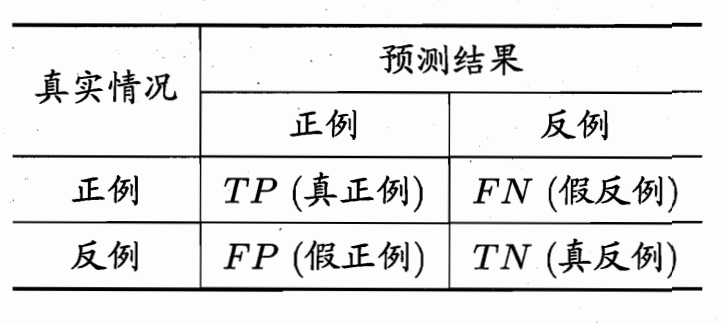
\includegraphics[scale=0.5]{../figures/RAMS1.PNG} 
\end{center}

查准率(也叫精度,precision)$P$与查全率(也叫召回率,recall)$R$定义为
\begin{eqnarray}
P=\frac{TP}{TP+FP}\\
R=\frac{TP}{TP+FN}
\end{eqnarray}
一般来说,查准率高时,查全率往往偏低,查全率高时,查准率往往偏低。

\paragraph{P-R曲线的绘制}对学习器的预测结果对样例进行排序,排在前面的是学习器认为“最可能”是正例的样本,排在最后的是学习器认为“最不可能”是正例的样本,按此顺序逐个把样本作为正例进行预测,则每次可以计算出当前的查全率、查准率,以查准率为纵轴,查全率为横轴作图,得到P-R曲线如下
\begin{center}
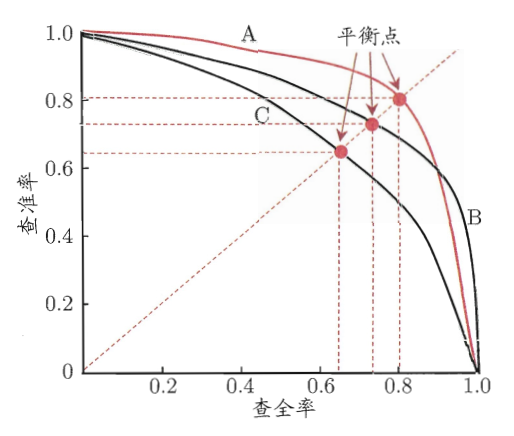
\includegraphics[scale=0.8]{../figures/RAMS2.PNG} 
\end{center}
若一个学习器的P-R曲线被另一个学习器的曲线完全“包住”,则可断言后者的性能优于前者。若两个学习器的P-R曲线有交叉点,则有以下的方法
\paragraph{平衡点(Break-Even Point,简称BEP)}它是“查准率=查全率”时的取值,如上图的学习器C的BEP为0.64,基于BEP的比较,认为学习器A优于B。
\paragraph{$F1$度量}BEP过于简化,通常用F1度量。F1是基于查准率与查全率的调和平均定义的
\begin{eqnarray}
\frac{1}{F1}=\frac{1}{2}\cdot(\frac{1}{P}+\frac{1}{R})
\end{eqnarray}
得到
\begin{eqnarray}
F1=\frac{2\times P\times R}{P+R}=\frac{2\times TP}{m+TP-TN}
\end{eqnarray}
其中,$m$为样例总数。
\paragraph{$F_\beta$度量}若对查准率和查全率重视程度不同,则用$F1$度量的一般形式:$F_\beta$,能让我们表达出对查准率、查全率的不同偏好,定义为
\begin{eqnarray}
F_\beta=\frac{(1+\beta^2)\times P\times R}{(\beta^2\times P)+R}
\end{eqnarray}
其中,$\beta>0$度量了查全率对查准率的相对重要性。$\beta=1$时退化为标准的$F1$,$\beta>1$时查全率有更大影响,$\beta<1$是查准率有更大影响。

很多时候会有多个混淆矩阵,有时进行多次的训练测试,或在多个数据集上进行训练测试,希望评估算法的“全局”性能,或是进行多分类任务。总之,是希望在$n$个二分类混淆矩阵上综合考察查准率和查全率。
\paragraph{宏查准率(macro-P)、宏查全率(macro-R)与宏F1(macro-F1)}先在各混淆矩阵上分别计算查准率和查全率,记为$(P_1,R_1),(P_2,R_2),\cdots,(P_n,R_n)$,再计算平均值
\begin{eqnarray}
macro-P&=&\frac{1}{n}\sum_{i=1}^nP_i\\
macro-R&=&\frac{1}{n}\sum_{i=1}^nR_i\\
macro-F1&=&\frac{2\times macro-P\times macro-R}{macro-P+macro-R}
\end{eqnarray}
\paragraph{微查准率(micro-P)、微查全率(micro-R)与微F1(micro-F1)}先在各混淆矩阵上分别计算查准率和查全率,记为$(P_1,R_1),(P_2,R_2),\cdots,(P_n,R_n)$,对混淆矩阵的对应元素进行平均,得到$TP,FP,TN,FN$的平均值,分别记为$\bar{TP},\bar{FP},\bar{TN},\bar{FN}$,再计算平均值
\begin{eqnarray}
micro-P&=&\frac{\bar{TP}}{\bar{TP}+\bar{FP}}\\
micro-R&=&\frac{\bar{TP}}{\bar{TP}+\bar{FN}}\\
micro-F1&=&\frac{2\times micro-P\times micro-R}{micro-P+micro-R}
\end{eqnarray}

\subsubsection{ROC与AUC}
\paragraph{ROC曲线的绘制}与P-R曲线相似,根据学习器的预测结果对样例进行排序,按此顺序逐个把样本作为正例进行预测,每次计算TPR和FPR的值,分别作为纵坐标、横坐标的值,就得到ROC曲线。ROC曲线的纵轴为真正例率(True Positive Rate,TRP),横轴为假正例率(False Positive Rate,FPR),定义如下
\begin{eqnarray}
TPR=\frac{TP}{TP+FN}\\
FPR=\frac{FP}{TN+FP}
\end{eqnarray}
\paragraph{有限样例的近似ROC曲线绘制}给定$m^+$个正例和$m^-$个反例,根据学习器预测结果对样例进行排序,然后把分类阈值设为最大,及把所有样例均预测为反例,此时真正例率和假正例率均为0,在坐标(0,0)处标记一个点,然后,将分类阈值依次设为每个样例的预测值,即依次将每个样例划分为正例。设前一个标记点坐标为$(x,y)$,当前若为真正例,则对应标记点的坐标为$(x,y+\frac{1}{m^+})$,若为假正例,则对应标记点的坐标为$(x+\frac{1}{m^-},y)$最后用线段连接相邻点即可。
\begin{center}
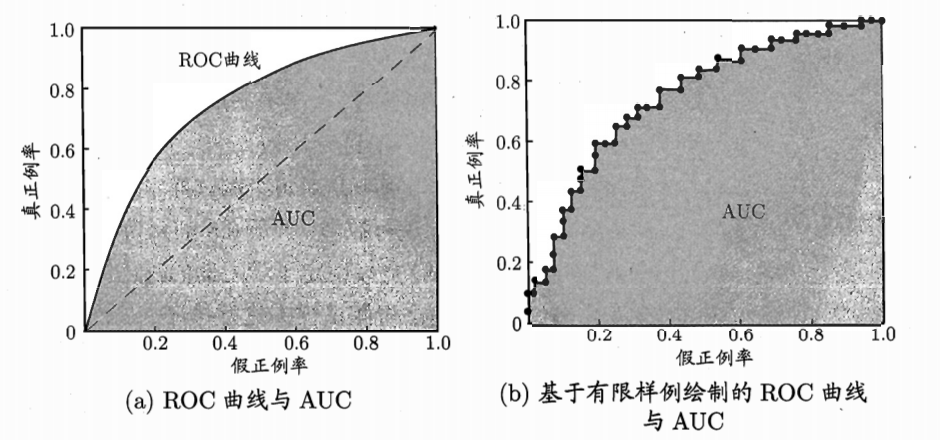
\includegraphics[scale=0.6]{../figures/RAMS3.PNG} 
\end{center}
若一个学习器的ROC曲线被另一个学习器的曲线完全“包住”,则可断言后者的性能优于前者。若两个学习器的ROC曲线有交叉点,则可比较ROC曲线下的面积,即AUC(Area Under ROC Curve)
\paragraph{AUC计算}假定ROC曲线是由坐标为$\{ (x_1,y_1),(x_2,y_2),\cdots,(x_m,y_m) \}$的点按序连接而形成(即$x_1=0,\cdots,x_m=1$),AUC可估算为
\begin{eqnarray}
AUC=\frac{1}{2}\sum_{i=1}^{m-1}(x_{i+1}-x_i)\cdot(y_i+y_{i+1})
\end{eqnarray}
给定$m^+$个正例和$m^-$个反例,令$D^+$和$D^-$分别表示正、反例集合,则排序“损失”(loss)定义为
\begin{eqnarray}
l_{rank}=\frac{1}{m^+m^-}\sum_{x^+\in D^+}\sum_{x^-\in D^-}
\left(
	1(f(x^+)<f(x^-))+\frac{1}{2}1(f(x^+)=f(x^-))
\right)
\end{eqnarray}

即考虑每一个正、反例,若正例的预测值小于反例,在记1个“罚分”,若相等,则记0.5个“罚分”。易得,$l_{rank}$对应的是ROC曲线之上的面积,若一个正例在ROC曲线上对应标记点的坐标为$(x,y)$,则$x$恰是排序在其之前的反例所占的比例,即假正例率,因此有
\begin{eqnarray}
AUC=1-l_{rank}
\end{eqnarray}

\subsubsection{代价敏感错误率与代价曲线}
以二分类为例,定义代价矩阵(cross matrix),其中$cost_{ij}$为第$i$类样本预测为第$j$类样本的代价。若将第0类判别为第1类所造成的损失更大,则$cost_{01}>cost_{10}$。代价矩阵如下
\begin{center}
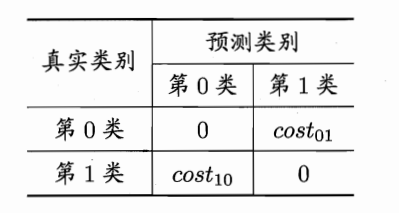
\includegraphics[scale=0.7]{../figures/RAMS4.PNG} 
\end{center}

在非均等代价下,目标不再是简单地最小化错误次数,而是最小化“总体代价”(total cost)







\subsection{特征选择}
对于一个有监督学习问题,数据的特征$n$很大,有可能为$n\gg m$,但是其中只有一小部分的特征是和学习任务相关的。当对$n$维的输入特征用简单的线性分类时,假设类的VC维将会是$O(n)$的,当训练数据不够大时,则过拟合是一个潜在的问题。于是,可以考虑采用特征选择算法来降低特征的数量。

\subsubsection{封装模型特征选择}
对于给定的$n$个特征,存在有$2^n$的可能的特征子集(因为特征有可能包含或不包含在子集中),因此特征选择转化为在$2^n$个可能的模型中的模型选择问题。对于一个很大的值$n$,计算和比较这$2^n$个模型将会变得很昂贵,所以采用启发式搜索的方法来寻找好的特征子集。这个搜索方法被称为前向搜索(forward search):
\begin{enumerate}[1]
\item 初始化$\mathcal{F}=\emptyset$
\item Repeat$\{$\\
\indent \ \ For $i=1,\cdots,n$\\
\indent \ \ \ \ (a)若$i\notin \mathcal{F}$,则令$\mathcal{F}_i=\mathcal{F}\cup\{i\}$,然后应用交叉验证的方法来评估特征$\mathcal{F}_i$(只使用$\mathcal{F}_i$中的特征来训练模型,并估计其泛化误差)
\\
\indent \ \ \ \ (b)将$\mathcal{F}$设为(a)中所找到的最优的特征子集$\}$
\item 经过如上循环而得到的最优特征子集。
\end{enumerate}

当$\mathcal{F}=\{1,2,\cdots,n\}$包含了所有的特征,或$\mathcal{F}$包含的特征数$\mathcal{F}$达到了一定的阈值(假设对特征数设置了最大值),算法的最外层循环将会终止。

上述的算法称为封装模型特征选择算法(wrapper model feature selection algorithm)。其含义是,我们“封装”了我们的算法模型,然后用不同的特征子集来估计算法的效果。除了前向搜索方法外,还有后向搜索方法,其与前项搜索方法的区别在于,其从$\mathcal{F}=\{1,2,\cdots,n\}$(包含所有特征)开始,然后重复删去特征,直到达到循环终止条件或$\mathcal{F}=\emptyset$。

封装模型特征选择算法通常情况下有好的效果,但是其多次调用学习算法会增大计算成本。实际上,完整的前向搜索算法,将会调用学习算法的次数为$O(n^2)$。

\subsubsection{过滤特征选择}
过滤特征选择提供了一种计算成本更小的选择特征子集的启发式算法。其思路是计算得分$S(i)$来度量特征$x_i$对类标签$y$的信息量。之后,只需找出$k$个得分最大的$S(i)$所对应的特征$i$。

一种定义$S(i)$的方式是基于训练集,计算$x_i$和$y$的协方差的绝对值,之后选择协方差绝对值大的几个特征作为最优特征子集。但有一种选择$S(i)$的更加常见的方法(尤其针对特征$x_i$为离散变量)为$x_i$和$y$之间的互信息(mutual information)$MI(x_i,y)$
\begin{eqnarray}
MI(x_i,y)=\sum_{x_i\in\{0,1\}}\sum_{y\in\{0,1\}}p(x_i,y)\log\frac{p(x_i,y)}{p(x_i)p(y)}
\end{eqnarray}
以上的方程假设$x_i$和$y_i$为二元分布。概率$P(x_i,y)$,$p(x_i)$,$p(y)$可以根据训练集的经验分布来估计。其也可以用KL散度(KUllback-leibler(KL)divergence)来表示
\begin{eqnarray}
MI(x_i,y)=KL(p(x_i,y)||p(x_i)p(y))
\end{eqnarray}

相对熵,又称为KL散度,是描述两个概率分布$P$和$Q$差异的一种方法,它是非对称的,这意味着$D(P||Q)\neq D(Q||P)$。在信息论中,$D(P||Q)$表示当用概率分布$Q$来拟合真实分布$P$时,产生的信息损耗,其中$P$表示真实分布,$Q$表示拟合分布。

设$P(x)$和$Q(x)$是$X$取值的两个离散概率分布,则$P$对$Q$的相对熵为
\begin{eqnarray}
D(P||Q)=\sum P(x)\log\frac{P(x)}{Q(x)}
\end{eqnarray}

于是,其给出了一种度量两个分布不同的方法。若$x_i$和$y$是独立随机变量,则有$p(x_i,y)=p(x_i)p(y)$,则这两个变量对应的分布的KL散度为0。因而若$x_i$和$y$是相互独立的,则可视为“$x_i$对$y$没有信息量”,因而得分$S(i)$很小。相反,若“$x_i$对$y$有信息量”,则其互信息$MI(x_i,y)$将是大的。

若已经根据得分$S(i)$对特征进行排序了,那么如何确定要选择的特征数目$k$?一种常规的方法是用交叉验证,在可能的值中选择$k$。例如,当利用朴素贝叶斯进行文本分类时,词汇量$n$通常会很大,使用这个方法来选择特征子集,将能够提高分类准确率。

\subsection{贝叶斯统计与规范化}
下面介绍一种用来克服过拟合的工具。我们采用最大化似然(maximum likelihood)来拟合参数,有
\begin{eqnarray}
\theta_{ML}=\arg\max_\theta\prod_{i=1}^mp(\sample{y}{i}|\sample{x}{i};\theta)
\end{eqnarray}
我们将$\theta$看作未知的参数。将$\theta$视为未知的但固定的参数是采用了频率学派统计学(frequentist statistics)的观点。在这个观点中,$\theta$不是随机的,只是其是未知的,于是我们的任务是通过统计学的方法(像极大似然估计)来估计参数。

另一种解决参数估计问题的方法是采用贝叶斯学派(Bayesian)的观点,然后把$\theta$视为一个随机变量。在这个方法中,我们对$\theta$确定一个先验分布(prior distribution)$p(\theta)$,来表达参数的先验信念(prior belief)。对于给定的训练集$S=\{ (\sample{x}{i},\sample{y}{i}) \}^m_{i=1}$当要对新的值$x$做预测时,我们可以先计算其后验分布(posterior distribution)
\begin{eqnarray}
\begin{aligned}
p(\theta|S)&=\frac{p(S|\theta) p(\theta)}{p(S)}\\
&= \frac{(\prod_{i=1}^mp(\sample{y}{i}|\sample{x}{i},\theta))p(\theta)}{\int_\theta (\prod_{i=1}^mp(\sample{y}{i}|\sample{x}{i},\theta)p(\theta))d\theta }
\end{aligned}
\end{eqnarray}
在上面的等式中,$p(\sample{y}{i}|\sample{x}{i},\theta)$来自所使用的模型。例如,若使用贝叶斯逻辑斯蒂回归,当$h_\theta(\sample{x}{i})=\frac{1}{1+e^{-\theta^T\sample{x}{i}}}$
则会选择$p(\sample{y}{i}|\sample{x}{i},\theta)=h_{\theta}(\sample{x}{i})^{\sample{y}{i}}(1-h_\theta (\sample{x}{i}))^{1-\sample{y}{i}}$

对于一个新的测试样例$x$,我们将用它做预测,我们可以基于在$\theta$的后延分布来计算在训练标签上的后验分布
\begin{eqnarray}
p(y|x,S)=\int_\theta p(y|x,\theta)p(\theta|S)d\theta
\end{eqnarray}
其中,$p(\theta|S)$来自上面,因此若目标是基于$x$来预测$y$,则可以得到
\begin{eqnarray}
E[y|x,S]=\int_yyp(y|x,S)dy
\end{eqnarray}
这个方法可以被视为 “完全贝叶斯(fully Bayesian)”预测。但实际上,后验分布很难计算,因为在求$p(\theta|S)$和计算后验概率时,需要完整的$\theta$的情况,因此其不可能算出解析解。

因此对$\theta$进行估计。一种方法是用点估计代替后验分布。用最大后验概率(maximum a posteriori)来估计$\theta$如下
\begin{eqnarray}
\theta_{MAP}=\arg\max_\theta\prod_{i=1}^mp(\sample{y}{i}|\sample{x}{i},\theta)p(\theta)
\end{eqnarray}
这个形式与对$\theta$最大似然估计相似,除了最后一项$p(\theta)$。

在应用中,可以将先验概率$p(\theta)$假设为服从$\theta\sim\mathcal{N}(0,\tau^2I)$。选择这种先验概率,拟合的参数$\theta_{MAP}$将会比使用最大似然要小,这也让贝叶斯MAP估计要比最大似然估计不容易过拟合。例如,贝叶斯逻辑斯蒂回归在文本分类上是一种高效的做法,虽然在文本分类中,通常会有$n\gg m$。









\section{附录}
\subsection{SVD分解}
假设$A$是一个$m\times n$的矩阵,可以分解为如下形式
\begin{eqnarray}
A = U\Sigma V^T
\end{eqnarray}
其中,$V$为$n\times n$的矩阵,如下定义
\begin{eqnarray}
(A^TA)v_i=\lambda_iv_i
\end{eqnarray}
$\lambda_i$为$A^TA$的特征值,$v_i$为$A^TA$的特征向量(为列向量)。$\Sigma$为$m\times n$的对角矩阵,对角元素为如下定义
\begin{eqnarray}
\Sigma_{ii}=\sqrt{\lambda_i}
\end{eqnarray}
$U$为$m\times m$的矩阵,定义为
\begin{eqnarray}
u_i=\frac{1}{\Sigma_{ii}}Av_i
\end{eqnarray}

上述$\sigma_i=\Sigma_{ii}$为奇异值,$u$为左奇异向量,奇异值在$\Sigma$中排列为从大到小,因此$\sigma$会减小地很快。多数情况下$10\%$甚至$1\%$的奇异值的和已经占了全部奇异值的和的$99\%$以上,因而可以选择前$r$个奇异值来近似地描述矩阵,定义\textbf{部分奇异值分解}:
\begin{eqnarray}
A_{m\times n}\approx U_{m\times r}\Sigma_{r\times r}V^T_{r\times n}
\end{eqnarray}
其中,$r$是一个远小于$m,n$的数。对于很大的矩阵$A$,储存将会耗费很大的空间,反而储存$U,S,V$是一个很好的选择。

\subsection{范数}
\subsubsection{常用向量范数}
对于$x=\vectornew{x}{n}^T$,则
\paragraph{p-范数}$||x||_p = (\sum_i^n |x_i|^p)^{\frac{1}{p}}$
\paragraph{1-范数}$||x||_1 = \sum_i^n |x_i|$
\paragraph{2-范数}$||x||_2 = (\sum_i^n |x_i|^2)^{\frac{1}{2}}$
\paragraph{$\infty$-范数}$||x||_p = \max\{|x_1|,\cdots,|x_n|\}$
\subsubsection{常用矩阵范数}
\paragraph{p-范数}$||A||_1=\max\{\sum|a_{i1}|,\sum|a_{i2}|,\cdots,\sum|a_{in}|\}$(列和范数,$A$每一列元素绝对值之和的最大值),其中$\sum|a_{i1}|$每一列元素绝对值的和$\sum|a_{i1}|=|a_{11}|+|a_{21}|+\cdots+|a_{n1}|$。
\paragraph{2-范数}$||A||_2=A$的最大奇异值$=(\max\{ \lambda_i(A^H*A) \})^\frac{1}{2}$(谱范数,即$A^H*A$特征值$\lambda_i$的平方根,其中$A^H$为$A$的共轭转置矩阵)
\paragraph{$\infty$-范数}$||A||_\infty=\max\{\sum|a_{1j}|,\sum|a_{2j}|,\cdots,\sum|a_{mj}|\}$(行和范数,$A$每一行元素绝对值之和的最大值),其中$\sum|a_{1j}|$每一列元素绝对值的和$\sum|a_{1j}|=|a_{11}|+|a_{12}|+\cdots+|a_{1m}|$
%if you like to use bibtex, you can delete the above line and use the following two lines
%\bibliographystyle{plain}
%\bibliography{YourFile/reference}
\end{document}
